% Author: Daniel Vartanian.
% Licence: MIT. See <https://opensource.org/license/mit/> to learn more.
% Based on: template.tex, developed by the Quarto team and
%   abtex2-modelo-trabalho-academico.tex, v-1.9.7, developed by
%   Lauro César Araujo and the team behind abnt2tex, with additional guidance
%   from the theses and dissertations regulations of the University of São Paulo
%   (USP). For more information, please visit <http://www.abntex.net.br/>.

% For help, see:
% * <https://quarto.org/docs/reference/formats/pdf.html>
% * <https://github.com/abntex/abntex2/wiki/ComoCustomizar>
% * <https://www.ctan.org/pkg/abntex2>
% * <https://www.ctan.org/pkg/memoir>
% * <https://www.ctan.org/pkg/hyperref>

% TODO:
% * Slightly move the toc to the left, in a way that the spacing between titles
%   and numbers become the same as the textual chapters.
% * Remove the hyperlink in the section numbering within TOC.
% * Remove hiperlink spans by page breaks. See: <https://tex.stackexchange.com/questions/54136/hyperref-link-spans-a-pagebreak-looks-ugly>.

% -----
% Preamble
% -----

\PassOptionsToPackage{
unicode
}{hyperref}

\PassOptionsToPackage{hyphens}{url}

\PassOptionsToPackage{dvipsnames,svgnames,x11names}{xcolor}


\documentclass[
12pt,
openright,
oneside,
a4paper,
chapter=TITLE,
section=TITLE,
french,
spanish,
brazil,
english
]{abntex2}\usepackage{array}
\usepackage{booktabs}
\usepackage{calc}
\usepackage{caption}
\usepackage{color}
\usepackage{colortbl}
\usepackage{amsmath}
\usepackage{amssymb}
\usepackage{booktabs}
\usepackage{enumitem}
\usepackage{etoolbox}
\usepackage{float}
\usepackage[T1]{fontenc}
\usepackage[hang]{footmisc}
\usepackage{graphicx}
\usepackage{iftex}
\usepackage{indentfirst}
\usepackage[utf8]{inputenc}
\usepackage{lastpage}
\usepackage{lipsum}
\usepackage{longtable}
\usepackage{microtype}
\usepackage{multirow}
\usepackage{parskip}
\usepackage{pdfpages}
\usepackage[table]{xcolor}

\usepackage{hyperref}

\ifPDFTeX
  \usepackage{textcomp} % provide euro and other symbols
\else % if luatex or xetex
  \usepackage{unicode-math}
\fi\newlength{\tinyskipamount}
\newlength{\hugeskipamount}

\setlength{\tinyskipamount}{0.5\baselineskip} % Arial/12pt/1.5 == 10.875pt
\setlength{\smallskipamount}{0.75\baselineskip} % Arial/12pt/1.5 == 16.3125pt
\setlength{\medskipamount}{1\baselineskip} % Arial/12pt/1.5 == 21.75pt
\setlength{\bigskipamount}{1.5\baselineskip} % Arial/12pt/1.5 == 32.625pt
\setlength{\hugeskipamount}{2\baselineskip }% Arial/12pt/1.5 == 43.5pt

\newcommand{\tinyskip}{\vspace{\tinyskipamount}}
\newcommand{\hugeskip}{\vspace{\hugeskipamount}}

\setlength{\beforechapskip}{\bigskipamount}
\setlength{\afterchapskip}{\smallskipamount}
\setbeforesecskip{\medskipamount}
\setaftersecskip{\smallskipamount}
\setbeforesubsecskip{\medskipamount}
\setaftersubsecskip{\smallskipamount}
\setbeforesubsubsecskip{\medskipamount}
\setaftersubsubsecskip{\smallskipamount}
\setbeforeparaskip{\medskipamount}
\setafterparaskip{0\smallskipamount}
% \setparahook{\addvspace{\smallskipamount}}% Set page -----

\setlength{\headsep}{1cm}
\setlength{\footskip}{1cm}
\checkandfixthelayout

% Set text spacing -----

\renewcommand{\familydefault}{\sfdefault}

\renewcommand{\baselinestretch}{1.5}

\setlength{\parindent}{1cm}

\setlength{\parskip}{0ex}

% Set text font -----


\ifPDFTeX\else
    % xetex/luatex font selection
  \setmainfont[]{Arial}
  \setsansfont[]{Arial}
  \setmonofont[ItalicFont=FragmentMono-Italic.otf,Scale=0.75]{FragmentMono-Regular.otf}




\fi


% Set page numbering -----

\makepagestyle{abntheadings}
\makeevenhead{abntheadings}{\ABNTEXfontereduzida\thepage}{}{}
\makeoddhead{abntheadings}{}{}{\ABNTEXfontereduzida\thepage}

% Set footnote -----

\setlength{\footnotemargin}{0.5em} % Equal to `\footmarkwidth`
\let\svfootnoterule\footnoterule % Equal to `\footmarksep`
\renewcommand\footnoterule{\svfootnoterule\vspace{1ex}}\newcommand{\capaname}{Capa}
\newcommand{\resumoestrangeironame}{Resumo}
\newcommand{\listadetermosname}{Lista de termos e definições}

\addto\captionsenglish{
  \renewcommand{\capaname}{Cover}
  \renewcommand{\folhaderostoname}{Title page}
  \renewcommand{\folhadeaprovacaoname}{Approval sheet}
  \renewcommand{\errataname}{Errata}
  \renewcommand{\dedicatorianame}{Inscription}
  \renewcommand{\agradecimentosname}{Acknowledgements}
  \renewcommand{\epigraphname}{Epigraph}
  \renewcommand{\resumoname}{Abstract}
  \renewcommand{\resumoestrangeironame}{Resumo}
  \renewcommand{\listfigurename}{List of figures}
  \renewcommand{\listtablename}{List of tables}
  \renewcommand{\listadesiglasname}{List of abbreviations and acronyms}
  \renewcommand{\listadesimbolosname}{List of symbols}
  \renewcommand{\listadetermosname}{List of terms and definitions}
  \renewcommand{\contentsname}{Contents}
  \renewcommand{\bibname}{References}
  \renewcommand{\apendicename}{APPENDIX}
  \renewcommand{\apendicesname}{Appendices}
  \renewcommand{\anexoname}{ANNEX}
  \renewcommand{\anexosname}{Annexes}
  \renewcommand{\indexname}{Index}
  \renewcommand{\orientadorname}{Supervisor:}
  \renewcommand{\coorientadorname}{Co-supervisor:}
  \renewcommand{\fontename}{Source}
  \renewcommand{\notaname}{Note}
  \renewcommand{\pageautorefname}{page}
  \renewcommand{\sectionautorefname}{section}
  \renewcommand{\subsectionautorefname}{subsection}
  \renewcommand{\subsubsectionautorefname}{subsubsection}
  \renewcommand{\paragraphautorefname}{subsubsubsection}
}

\addto\captionsbrazil{
  \renewcommand{\capaname}{Capa}
  \renewcommand{\folhaderostoname}{Página de título}
  \renewcommand{\folhadeaprovacaoname}{Folha de aprovação}
  \renewcommand{\errataname}{Errata}
  \renewcommand{\dedicatorianame}{Dedicatória}
  \renewcommand{\agradecimentosname}{Agradecimentos}
  \renewcommand{\epigraphname}{Epígrafe}
  \renewcommand{\resumoname}{Resumo}
  \renewcommand{\resumoestrangeironame}{Abstract}
  \renewcommand{\listfigurename}{Lista de figuras}
  \renewcommand{\listtablename}{Lista de tabelas}
  \renewcommand{\listadesiglasname}{Lista de abreviaturas e siglas}
  \renewcommand{\listadesimbolosname}{Lista de símbolos}
  \renewcommand{\listadetermosname}{Lista de termos e definições}
  \renewcommand{\contentsname}{Sumário}
  \renewcommand{\bibname}{Referências}
  \renewcommand{\apendicename}{APÊNDICE}
  \renewcommand{\apendicesname}{Apêndices}
  \renewcommand{\anexoname}{ANEXO}
  \renewcommand{\anexosname}{Anexos}
  \renewcommand{\indexname}{Índice}
  \renewcommand{\orientadorname}{Asesor:}
  \renewcommand{\coorientadorname}{Coasesor:}
  \renewcommand{\sourcename}{Fuente}
  \renewcommand{\notaname}{Nota}
  \renewcommand{\pageautorefname}{página}
  \renewcommand{\sectionautorefname}{sección}
  \renewcommand{\subsectionautorefname}{subsección}
  \renewcommand{\subsubsectionautorefname}{subsubsección}
  \renewcommand{\paragraphautorefname}{subsubsubsección}
}

\addto\captionsspanish{
  \renewcommand{\capaname}{Portada}
  \renewcommand{\folhaderostoname}{Página de título}
  \renewcommand{\folhadeaprovacaoname}{Hoja de aprobación}
  \renewcommand{\errataname}{Errata}
  \renewcommand{\dedicatorianame}{Dedicatoria}
  \renewcommand{\agradecimentosname}{Agradecimientos}
  \renewcommand{\epigraphname}{Epígrafe}
  \renewcommand{\resumoname}{Resumen}
  \renewcommand{\resumoestrangeironame}{Resumo}
  \renewcommand{\listfigurename}{Lista de figuras}
  \renewcommand{\listtablename}{Lista de tablas}
  \renewcommand{\listadesiglasname}{Lista de abreviaturas y siglas}
  \renewcommand{\listadesimbolosname}{Lista de símbolos}
  \renewcommand{\listadetermosname}{Lista de términos y definiciones}
  \renewcommand{\contentsname}{Sumario}
  \renewcommand{\bibname}{Referencias}
  \renewcommand{\apendicename}{APÉNDICE}
  \renewcommand{\apendicesname}{Apéndices}
  \renewcommand{\anexoname}{ANEXO}
  \renewcommand{\anexosname}{Anexos}
  \renewcommand{\indexname}{Índice}
  \renewcommand{\orientadorname}{Asesor:}
  \renewcommand{\coorientadorname}{Coasesor:}
  \renewcommand{\sourcename}{Fuente}
  \renewcommand{\notaname}{Nota}
  \renewcommand{\pageautorefname}{página}
  \renewcommand{\sectionautorefname}{sección}
  \renewcommand{\subsectionautorefname}{subsección}
  \renewcommand{\subsubsectionautorefname}{subsubsección}
  \renewcommand{\paragraphautorefname}{subsubsubsección}
}

\addto\captionsfrench{
  \renewcommand{\capaname}{Couverture}
  \renewcommand{\folhaderostoname}{Page de titre}
  \renewcommand{\folhadeaprovacaoname}{Feuille d'approbation}
  \renewcommand{\errataname}{Errata}
  \renewcommand{\dedicatorianame}{Dédiace
  \renewcommand{\agradecimentosname}{Remerciements}}
  \renewcommand{\epigraphname}{Épigraphe}
  \renewcommand{\resumoname}{Résumé}
  \renewcommand{\resumoestrangeironame}{Resumo}
  \renewcommand{\listfigurename}{Liste des figures}
  \renewcommand{\listtablename}{Liste des tableaux}
  \renewcommand{\listadesiglasname}{Liste des abréviations et sigles}
  \renewcommand{\listadesimbolosname}{Liste des symboles}
  \renewcommand{\listadetermosname}{Liste des termes et définitions}
  \renewcommand{\contentsname}{Sommaire}
  \renewcommand{\bibname}{Références}
  \renewcommand{\apendicename}{APPENDICE}
  \renewcommand{\apendicesname}{Appendices}
  \renewcommand{\anexoname}{ANNEXE}
  \renewcommand{\anexosname}{Annexes}
  \renewcommand{\indexname}{Index}
  \renewcommand{\orientadorname}{Conseiller:}
  \renewcommand{\coorientadorname}{Co-conseiller:}
  \renewcommand{\sourcename}{Source}
  \renewcommand{\notaname}{Note}
  \renewcommand{\pageautorefname}{page}
  \renewcommand{\sectionautorefname}{section}
  \renewcommand{\subsectionautorefname}{sous-section}
  \renewcommand{\subsubsectionautorefname}{sous-sous-section}
  \renewcommand{\paragraphautorefname}{sous-sous-sous-section}
}% Set text variables -----

\renewcommand{\ABNTEXchapterfont}{\normalfont\bfseries}
\renewcommand{\ABNTEXchapterfontsize}{\normalsize}
\renewcommand{\ABNTEXsectionfont}{\normalfont}
\renewcommand{\ABNTEXsectionfontsize}{\normalsize}
\renewcommand{\ABNTEXsubsectionfont}{\normalfont\bfseries}
\renewcommand{\ABNTEXsubsectionfontsize}{\normalsize}
\renewcommand{\ABNTEXsubsubsectionfont}{\normalfont}
\renewcommand{\ABNTEXsubsubsectionfontsize}{\normalsize}
\renewcommand{\ABNTEXsubsubsubsectionfont}{\normalfont}
\renewcommand{\ABNTEXsubsubsubsectionfontsize}{\normalsize\itshape}
\renewcommand{\ABNTEXfontereduzida}{\footnotesize}

\renewcommand{\chapnumfont}{\normalfont}
\renewcommand{\captiontitlefont}{\ABNTEXfontereduzida}

\renewcommand{\ABNTEXcaptiondelim}{~\textendash~}
\renewcommand{\ABNTEXcaptionfontedelim}{:~}

% Set new commands

\providecommand{\imprimiruniversidade}{}
\newcommand{\universidade}[1]{\renewcommand{\imprimiruniversidade}{#1}}

\providecommand{\imprimirescola}{}
\newcommand{\escola}[1]{\renewcommand{\imprimirescola}{#1}}

\providecommand{\imprimirprograma}{}
\newcommand{\programa}[1]{\renewcommand{\imprimirprograma}{#1}}

\newcommand{\imprimirtipodetrabalho}{\imprimirtipotrabalho}

\providecommand{\imprimirtipodetituloacademico}{}
\newcommand{\tipodetituloacademico}[1]{\renewcommand{\imprimirtipodetituloacademico}{#1}}

\providecommand{\imprimirtituloacademico}{}
\newcommand{\tituloacademico}[1]{\renewcommand{\imprimirtituloacademico}{#1}}

\providecommand{\imprimirareadeconcentracao}{}
\newcommand{\areadeconcentracao}[1]{\renewcommand{\imprimirareadeconcentracao}{#1}}

\providecommand{\imprimirnotadeversao}{}
\newcommand{\notadeversao}[1]{\renewcommand{\imprimirnotadeversao}{#1}}

% Set chapter/section formating -----

\setsecnumformat{\normalfont\csname the#1\endcsname\quad}

\renewcommand{\printchapternum}{
  \tocprintchapter
  \setboolean{abntex@innonumchapter}{false}
  \chapnumfont
  \thechapter \quad
  \ifthenelse{\boolean{abntex@apendiceousecao}}{
      \tocinnonumchapter
      \ABNTEXcaptiondelim
  }{}
}

% Similar to `\printloftitle`
\renewcommand{\pretextualchapter}[1]{
  \setlength{\afterchapskip}{\hugeskipamount}
  \addtocounter{abntex@bookmarkcounter}{1}
  \PRIVATEbookmarkthis{#1}
  \chapter*[#1]{#1}
}

\makechapterstyle{apendice}{
  \setlength{\beforechapskip}{-\baselineskip}
  \setlength{\midchapskip}{0\baselineskip}
  \setlength{\afterchapskip}{\smallskipamount}
  \renewcommand{\chapnamefont}{\normalfont}
  \renewcommand{\printchaptername}{\ABNTEXchapterupperifneeded{\appendixname}}
  \renewcommand{\chapternamenum}{\space}
  \renewcommand{\chapnumfont}{\normalfont}
  \renewcommand{\printchapternum}{\thechapter}
  \renewcommand{\afterchapternum}{\space -- \space}
  \renewcommand{\chaptitlefont}{\normalfont}
  \renewcommand{\printchaptertitle}[1]{\ABNTEXchapterupperifneeded{##1}}
  \renewcommand{\afterchaptertitle}{\vspace{\smallskipamount}}
}

% Set `\textual` -----

\renewcommand{\textual}{
  \pagestyle{abntheadings}
  \aliaspagestyle{chapter}{abntheadings}
}

% Set cover -----

\renewcommand{\imprimircapa}{
  \phantomsection\pdfbookmark[0]{\capaname}{}
  \begin{capa}%
  \begin{adjustwidth}{-1cm}{0cm}
  \center
  \imprimirinstituicao
  \vfill

  \imprimirautor
  \vfill

  \textbf{\imprimirtitulo}
  \vspace{10cm}

  \imprimirlocal

  \imprimirdata
  \vspace{1.5cm}
  \end{adjustwidth}
  \end{capa}
}

% Set title page -----

\makeatletter
\renewcommand{\folhaderostocontent}{
  \begin{center}
  \imprimirautor
  \vfill

  \bfseries\imprimirtitulo
  \vfill

  \bfseries\imprimirnotadeversao\normalfont
  \vfill

  \abntex@ifnotempty{
    \imprimirpreambulo
  }{
    \hspace{0.35\textwidth}
    \begin{minipage}{.6\textwidth}
    \SingleSpacing
    \imprimirpreambulo
    \end{minipage}
  }
  \vfill

  \imprimirlocal

  \imprimirdata
  \vspace{1cm}
  \end{center}
}
\makeatother

% Set cataloging record -----

\renewenvironment{fichacatalografica}{
  \setlength{\parindent}{0cm}
  \begin{SingleSpacing}
}{
  \end{SingleSpacing}%
}

% Set errata -----

\renewenvironment{errata}[1][\errataname]{
  \pretextualchapter{#1}
  % \setlength{\parindent}{0cm}
}{
  \cleardoublepage
}

% Set approval sheet -----

\renewenvironment{folhadeaprovacao}[1][\folhadeaprovacaoname]{
  \clearpage
  \PRIVATEbookmarkthis{#1}
  \setlength\parindent{0cm}
  \AtBeginEnvironment{tabular}{\normalsize}
  \begin{SingleSpace}
}{
  \end{SingleSpace}
  \cleardoublepage
}

% Set abstract -----

\newenvironment{resumoenv}[1][\resumoname]{
  % \pretextualchapter{#1}
  \setlength{\afterchapskip}{\hugeskipamount - \smallskipamount}
  \addtocounter{abntex@bookmarkcounter}{1}
  \PRIVATEbookmarkthis{#1}
  \chapter*[#1]{#1}

  \setlength{\parindent}{0cm}
  \setlength{\parskip}{\smallskipamount} % The troublemaker.
  \AtBeginEnvironment{tabular}{\normalsize}
  \renewcommand{\arraystretch}{1}
  \setlength{\aboverulesep}{0ex}
  \setlength{\belowrulesep}{0ex}
  \setlength{\arrayrulewidth}{0pt}
  \setlength{\tabcolsep}{0cm}
  \begin{SingleSpace}
}{
  \end{SingleSpace}
  \cleardoublepage
}

% Set list of abbreviations and acronyms -----

\renewenvironment{siglas}{
  \pretextualchapter{\listadesiglasname}
}{
  \cleardoublepage
}

% Set list of symbols -----

\renewenvironment{simbolos}{
  \pretextualchapter{\listadesimbolosname}
}{
  \cleardoublepage
}
% Set list of symbols -----

\newenvironment{termos}{%
  \pretextualchapter{\listadetermosname}
}{
  \cleardoublepage
}

% Set appendices and annexes -----

\renewcommand{\PRIVATEapendiceconfig}[1]{
  \setboolean{abntex@apendiceousecao}{true}
  \renewcommand{\appendixname}{#1}
  \renewcommand{\apendicesname}{#1}
  \switchchapname{#1}

  % Note:
  %
  % \cleardoublepage
  % \phantomsection
  % \addcontentsline{toc}{part}{Appendices}
  % \appendix
  %
  % is automatically add by the Quarto render.
}

\newcommand{\PRIVATEannexconfig}[2]{
  \setboolean{abntex@apendiceousecao}{true}
  \renewcommand{\appendixname}{#1}
  \renewcommand{\apendicesname}{#1}
  \renewcommand{\appendixtocname}{#2}
  \phantomsection
  \addcontentsline{toc}{part}{\appendixtocname}
  \switchchapname{#1}
}

\renewcommand{\apendices}{
  \cftinserthook{toc}{appendixhook}
  \PRIVATEapendiceconfig{\apendicename}
  \appendix
  \chapterstyle{apendice}
}

\renewenvironment{apendicesenv}{
  \cftinserthook{toc}{appendixhook}
  \PRIVATEapendiceconfig{\apendicename}
  \begin{appendix}
  \chapterstyle{apendice}
}{
  \end{appendix}
  \setboolean{abntex@apendiceousecao}{false}
  \bookmarksetup{startatroot}
}

\renewcommand{\anexos}{
  \cftinserthook{toc}{appendixhook}
  \PRIVATEannexconfig{\anexoname}{\anexosname}
  \appendix
  \renewcommand\theHchapter{anexochapback.\arabic{chapter}}
  \chapterstyle{apendice}
}

\renewenvironment{anexosenv}{
  \cftinserthook{toc}{appendixhook}
  \PRIVATEannexconfig{\anexoname}{\anexosname}
  \begin{appendix}
  \renewcommand\theHchapter{anexochapback.\arabic{chapter}}
  \chapterstyle{apendice}
}{
  \end{appendix}
  \setboolean{abntex@apendiceousecao}{false}
  \bookmarksetup{startatroot}
}

% Set index section -----

\definecolor{blue}{HTML}{2905C3}

% See <https://getbootstrap.com/docs/4.0/utilities/colors/>.
\definecolor{quarto-blue}{HTML}{2780E3}
\definecolor{quarto-lighter-blue}{HTML}{ECF4FC}
\definecolor{quarto-orange}{HTML}{FF7518}
\definecolor{quarto-ligther-orange}{HTML}{FFF3EB}
\definecolor{quarto-red}{HTML}{D9534F}
\definecolor{quarto-ligther-red}{HTML}{FCF1F1}
\definecolor{quarto-green}{HTML}{3FB618}
\definecolor{quarto-ligther-green}{HTML}{EFF9EB}
\definecolor{quarto-purple}{HTML}{7D12BA}
\definecolor{quarto-gray}{HTML}{A3A3A3}
\definecolor{quarto-medium-gray}{HTML}{CFD0D1}
\definecolor{quarto-ligther-gray}{HTML}{F1F3F5}

\definecolor{bs-link-color}{HTML}{39729E}% \usepackage{graphicx}
\makeatletter
\def\maxwidth{\ifdim\Gin@nat@width>\linewidth\linewidth\else\Gin@nat@width\fi}
\def\maxheight{\ifdim\Gin@nat@height>\textheight\textheight\else\Gin@nat@height\fi}
\makeatother

% Scale images if necessary, so that they will not overflow the page
% margins by default, and it is still possible to overwrite the defaults
% using explicit options in \includegraphics[width, height, ...]{}
\setkeys{Gin}{width=\maxwidth,height=\maxheight,keepaspectratio}

% Set default figure placement to htbp
\makeatletter
\def\fps@figure{htbp}
\makeatother

\makeatletter
\setlength{\@fptop}{5pt} % Set distance from top of page to first float
\makeatother

\captionsetup{
  font=footnotesize, % Must be `\ABNTEXfontereduzida` equivalent.
  justification=centering,
  skip=16.3125pt % Skip between caption and figure (`0.75\baselineskip`).
}

\renewcommand{\legend}[1]{
  \addvspace{0.75\baselineskip}
  \ABNTEXfontereduzida \raggedright #1
}

% % Credits: <https://stackoverflow.com/a/1566053/8258804>.
% \makeatletter
% \let\oldfigure\figure
% \def\figure{\@ifnextchar[\figure@i \figure@ii}
% \def\figure@i[#1]{\oldfigure[#1]\centering}
% \def\figure@ii{\oldfigure\centering}
% \makeatother\renewcommand{\arraystretch}{1}
\setlength{\aboverulesep}{0ex}
\setlength{\belowrulesep}{0ex}

% Correct order of tables after \paragraph or \subparagraph
\usepackage{etoolbox}
\makeatletter
\patchcmd\longtable{\par}{\if@noskipsec\mbox{}\fi\par}{}{}
\makeatother

% Allow footnotes in longtable head/foot
\IfFileExists{footnotehyper.sty}{\usepackage{footnotehyper}}{\usepackage{footnote}}
\makesavenoteenv{longtable}

% Set tabular environment -----

% \providecommand{\addquartolegend}{}
% \newcommand{\quartolegend}[1]{\renewcommand{\addquartolegend}{#1}}
% \renewcommand{\quartolegend}{Don't forget to set \verb|\quartolegend|!}

\AtBeginEnvironment{table}{\ABNTEXfontereduzida}
\AtBeginEnvironment{tabular}{\ABNTEXfontereduzida}

\AddToHook{env/longtable/before}{}
\AddToHook{env/longtable/after}{}
\AddToHook{env/longtable/begin}{
  \ABNTEXfontereduzida
  \renewcommand{\arraystretch}{1}
}
\AddToHook{env/longtable/end}{}

\floatplacement{table}{H}\providecommand{\tightlist}{
\setlength{\itemsep}{0pt}\setlength{\parskip}{0pt}}\makeatletter
\newcommand*{\getlength}[1]{\strip@pt#1}
\makeatother\title{\{abnt\}: Quarto format for ABNT theses and
dissertations}
\titulo{\{abnt\}: Quarto format for ABNT theses and dissertations}


\author{Daniel Vartanian}
\autor{Daniel Vartanian}

\local{{[}City{]}}

\date{2023}
\data{2023}

\orientador{{[}Supervisor's full name{]}}

\coorientador{{[}Co-supervisor's full name{]}}

\tipodetituloacademico{{[}Master/PhD{]}}

\tituloacademico{{[}Master of Science/Doctor of Science{]}}

\tipotrabalho{{[}Dissertation/Thesis{]}}

\areadeconcentracao{{[}Area of concentration{]}}

\instituicao{\MakeUppercase{{[}University{]}}}
\universidade{{[}University{]}}

\instituicao{
  \MakeUppercase{{[}University{]}}
  \par
  \MakeUppercase{{[}School/Department{]}}
}

\escola{{[}School/Department{]}}

\instituicao{
  \MakeUppercase{{[}University{]}}
  \par
  \MakeUppercase{{[}School/Department{]}}
  \par
  \MakeUppercase{{[}Graduate program{]}}
}

\programa{{[}Graduate program{]}}

\notadeversao{{[}Original/Revised version{]}}
\hypersetup{
pdftitle={\{abnt\}: Quarto format for ABNT theses and dissertations},
pdfauthor={Daniel Vartanian},
pdflang={en},
pdfsubject={{[}Dissertation/Thesis{]}},
linktoc={section},
colorlinks=true,
linkcolor={blue},
filecolor={blue},
citecolor={blue},
urlcolor={blue},
pdfcreator={LaTeX via pandoc},
bookmarksdepth=5
}% Set LoF -----

\renewcommand{\printloftitle}[1]{
  % Do not use `\pretextualchapter` here. It'll make a duplicated bookmark.
  \setlength{\afterchapskip}{
    \hugeskipamount - 18pt % It is what it is...
  }

  \chapter*[#1]{#1}
}

% Set LoT -----

\renewcommand{\printlottitle}[1]{
  % Do not use `\pretextualchapter` here. It'll make a duplicated bookmark.
  \setlength{\afterchapskip}{
    \hugeskipamount - 18pt % It is what it is...
  }

  \chapter*[#1]{#1}
}

% Set ToC -----

\renewcommand{\aftertoctitle}{
  \center
  \vspace{\hugeskipamount - 16pt} % It is what it is...
}

\setlength{\cftpartindent}{6em}
\setlength{\cftsectionnumwidth}{6em}
\setlength{\cftsubsectionnumwidth}{6em}
\setlength{\cftsubsubsectionnumwidth}{6em}
\setlength{\cftparagraphnumwidth}{6em}

\setlength{\cftbeforebookskip}{0pt}
\setlength{\cftbeforepartskip}{2em}
\setlength{\cftbeforechapterskip}{0.5em}
\setlength{\cftbeforesectionskip}{0pt}
\setlength{\cftbeforesubsectionskip}{0pt}
\setlength{\cftbeforesubsubsectionskip}{0pt}
\setlength{\cftbeforeparagraphskip}{0pt}

\renewcommand{\cftchapterpresnum}{\normalfont}
\renewcommand{\cftchapteraftersnum}{\normalfont}
\renewcommand{\cftchapteraftersnumb}{\normalfont\normalsize\bfseries\hspace{0.87em}}
\renewcommand{\cftsubsectionpresnum}{\normalfont}
\renewcommand{\cftparagraphpresnum}{\normalfont}

\renewcommand{\cftpartfont}{\normalfont\normalsize\bfseries\MakeUppercase}
\renewcommand{\cftchapterfont}{\normalfont\normalsize\bfseries\MakeUppercase}
\renewcommand{\cftsectionfont}{\normalfont\normalsize\MakeUppercase}
\renewcommand{\cftsubsectionfont}{\normalfont\normalsize\bfseries}
\renewcommand{\cftsubsubsectionfont}{\normalfont\normalsize}
\renewcommand{\cftparagraphfont}{\normalfont\normalsize\itshape}

\renewcommand{\cftpartpagefont}{\normalfont\normalsize}
\renewcommand{\cftchapterpagefont}{\normalfont\normalsize}
\renewcommand{\cftsectionpagefont}{\normalfont\normalsize}
\renewcommand{\cftsubsectionpagefont}{\normalfont\normalsize}
\renewcommand{\cftsubsubsectionpagefont}{\normalfont\normalsize}
\renewcommand{\cftparagraphpagefont}{\normalfont\normalsize}
\renewcommand{\cftfigurepagefont}{\normalfont\normalsize}
\renewcommand{\cfttablepagefont}{\normalfont\normalsize}

\cftinsertcode{bibhook}{
  \setlength{\cftchapterindent}{5.675em}
  \setlength{\cftchapternumwidth}{0em}
  \renewcommand{\cftchapteraftersnumb}{\hspace{0em}}
  \renewcommand{\cftchapterpresnum}{\normalfont\bfseries}
}

\cftinsertcode{appendixhook}{
    \setlength{\cftchapterindent}{6em} %
    \renewcommand{\cftchaptername}{\appendixname\space}
    \setlength{\cftchapternumwidth}{2.3em} % check
    \renewcommand{\cftchapteraftersnumb}{
        \hspace{-1.5em} -- \space % check \hspace{-1.5em}
    }
}\usepackage[
style=abnt,backend=biber,,language=english,,url=true,,useprefix=false,,giveninits=true,,extrayear=true
]{biblatex}

\usepackage{csquotes}

\addbibresource{references.bib}

\renewcommand{\bibname}{REFERENCES}
\newcommand{\newbibname}{REFERENCES}


\newcommand{\bibnamewithfootnote}{
  \newbibname\protect\footnote{According to the Brazilian Association of
Technical Standards (ABNT NBR 6023).}
}

\setlength{\bibhang}{0cm}

\setlength{\bibparsep}{0ex}


\defbibheading{bibheading}[\bibnamewithfootnote]{
  \ifthenelse{\boolean{ABNTEXupperchapter}}{
    \setboolean{ABNTEXupperchapter}{false}
    \chapter*{#1}
    \markboth{#1}{#1}
    \setboolean{ABNTEXupperchapter}{true}
  }{
    \chapter*{#1}
    \markboth{#1}{#1}
  }
}


\AtBeginBibliography{
  \vspace{\hugeskipamount - 2.9pt} % It is what it is...
}

\AtEveryBibitem{\clearfield{annotation}}
\renewcommand{\bibfont}{\ABNTEXfontereduzida}% Use upquote if available, for straight quotes in verbatim environments
\IfFileExists{upquote.sty}{\usepackage{upquote}}{}
\IfFileExists{microtype.sty}{% use microtype if available
  \usepackage[]{microtype}
  \UseMicrotypeSet[protrusion]{basicmath} % disable protrusion for tt fonts
}{}





\setlength{\emergencystretch}{3em} % Prevent overfull lines

\setcounter{secnumdepth}{5}

% Make \paragraph and \subparagraph free-standing
\ifx\paragraph\undefined\else
  \let\oldparagraph\paragraph
  \renewcommand{\paragraph}[1]{\oldparagraph{#1}\mbox{}}
\fi
\ifx\subparagraph\undefined\else
  \let\oldsubparagraph\subparagraph
  \renewcommand{\subparagraph}[1]{\oldsubparagraph{#1}\mbox{}}
\fi

\usepackage{color}
\usepackage{fancyvrb}
\newcommand{\VerbBar}{|}
\newcommand{\VERB}{\Verb[commandchars=\\\{\}]}
\DefineVerbatimEnvironment{Highlighting}{Verbatim}{commandchars=\\\{\}}
% Add ',fontsize=\small' for more characters per line
\usepackage{framed}
\definecolor{shadecolor}{RGB}{241,243,245}
\newenvironment{Shaded}{\begin{snugshade}}{\end{snugshade}}
\newcommand{\AlertTok}[1]{\textcolor[rgb]{0.68,0.00,0.00}{#1}}
\newcommand{\AnnotationTok}[1]{\textcolor[rgb]{0.37,0.37,0.37}{#1}}
\newcommand{\AttributeTok}[1]{\textcolor[rgb]{0.40,0.45,0.13}{#1}}
\newcommand{\BaseNTok}[1]{\textcolor[rgb]{0.68,0.00,0.00}{#1}}
\newcommand{\BuiltInTok}[1]{\textcolor[rgb]{0.00,0.23,0.31}{#1}}
\newcommand{\CharTok}[1]{\textcolor[rgb]{0.13,0.47,0.30}{#1}}
\newcommand{\CommentTok}[1]{\textcolor[rgb]{0.37,0.37,0.37}{#1}}
\newcommand{\CommentVarTok}[1]{\textcolor[rgb]{0.37,0.37,0.37}{\textit{#1}}}
\newcommand{\ConstantTok}[1]{\textcolor[rgb]{0.56,0.35,0.01}{#1}}
\newcommand{\ControlFlowTok}[1]{\textcolor[rgb]{0.00,0.23,0.31}{#1}}
\newcommand{\DataTypeTok}[1]{\textcolor[rgb]{0.68,0.00,0.00}{#1}}
\newcommand{\DecValTok}[1]{\textcolor[rgb]{0.68,0.00,0.00}{#1}}
\newcommand{\DocumentationTok}[1]{\textcolor[rgb]{0.37,0.37,0.37}{\textit{#1}}}
\newcommand{\ErrorTok}[1]{\textcolor[rgb]{0.68,0.00,0.00}{#1}}
\newcommand{\ExtensionTok}[1]{\textcolor[rgb]{0.00,0.23,0.31}{#1}}
\newcommand{\FloatTok}[1]{\textcolor[rgb]{0.68,0.00,0.00}{#1}}
\newcommand{\FunctionTok}[1]{\textcolor[rgb]{0.28,0.35,0.67}{#1}}
\newcommand{\ImportTok}[1]{\textcolor[rgb]{0.00,0.46,0.62}{#1}}
\newcommand{\InformationTok}[1]{\textcolor[rgb]{0.37,0.37,0.37}{#1}}
\newcommand{\KeywordTok}[1]{\textcolor[rgb]{0.00,0.23,0.31}{#1}}
\newcommand{\NormalTok}[1]{\textcolor[rgb]{0.00,0.23,0.31}{#1}}
\newcommand{\OperatorTok}[1]{\textcolor[rgb]{0.37,0.37,0.37}{#1}}
\newcommand{\OtherTok}[1]{\textcolor[rgb]{0.00,0.23,0.31}{#1}}
\newcommand{\PreprocessorTok}[1]{\textcolor[rgb]{0.68,0.00,0.00}{#1}}
\newcommand{\RegionMarkerTok}[1]{\textcolor[rgb]{0.00,0.23,0.31}{#1}}
\newcommand{\SpecialCharTok}[1]{\textcolor[rgb]{0.37,0.37,0.37}{#1}}
\newcommand{\SpecialStringTok}[1]{\textcolor[rgb]{0.13,0.47,0.30}{#1}}
\newcommand{\StringTok}[1]{\textcolor[rgb]{0.13,0.47,0.30}{#1}}
\newcommand{\VariableTok}[1]{\textcolor[rgb]{0.07,0.07,0.07}{#1}}
\newcommand{\VerbatimStringTok}[1]{\textcolor[rgb]{0.13,0.47,0.30}{#1}}
\newcommand{\WarningTok}[1]{\textcolor[rgb]{0.37,0.37,0.37}{\textit{#1}}}

\newcolumntype{P}[1]{>{\centering\arraybackslash}p{#1}}

\clubpenalty10000
\widowpenalty10000
\displaywidowpenalty10000

\ifLuaTeX
  \usepackage{selnolig}  % disable illegal ligatures
\fi


\IfFileExists{xurl.sty}{\usepackage{xurl}}{} % add URL line breaks if available
\urlstyle{same} % disable monospaced font for URLs


%:::% class attribute begin/end %:::%

% -----
% Title page
% -----

%:::% title-page begin %:::%
\preambulo{
%:::% title-page body begin %:::%
{\imprimirtipotrabalho} presented to the {\imprimirescola} at {\imprimiruniversidade}, as part of the requirements for the degree of {\imprimirtituloacademico} by the {\imprimirprograma}.
\tinyskip

Area of concentration: {\imprimirareadeconcentracao}.
\tinyskip

Revised version incorporating the changes requested by the examining committee on [Date]. The original version is held in the reserved collection at the {\imprimirescola} Library and in the Digital Library of Theses and Dissertations of the {\imprimiruniversidade}.
\tinyskip

Supervisor: Prof. Dr. {\imprimirorientador}
\vspace{0.25\baselineskip}

Co-Supervisor: Prof. Dr. {\imprimircoorientador}
%:::% title-page body end %:::%
}
%:::% title-page end %:::%
\usepackage{booktabs}
\usepackage{caption}
\usepackage{longtable}
\usepackage{colortbl}
\usepackage{array}
\makeatletter
\@ifpackageloaded{tcolorbox}{}{\usepackage[skins,breakable]{tcolorbox}}
\@ifpackageloaded{fontawesome5}{}{\usepackage{fontawesome5}}
\definecolor{quarto-callout-color}{HTML}{909090}
\definecolor{quarto-callout-note-color}{HTML}{0758E5}
\definecolor{quarto-callout-important-color}{HTML}{CC1914}
\definecolor{quarto-callout-warning-color}{HTML}{EB9113}
\definecolor{quarto-callout-tip-color}{HTML}{00A047}
\definecolor{quarto-callout-caution-color}{HTML}{FC5300}
\definecolor{quarto-callout-color-frame}{HTML}{acacac}
\definecolor{quarto-callout-note-color-frame}{HTML}{4582ec}
\definecolor{quarto-callout-important-color-frame}{HTML}{d9534f}
\definecolor{quarto-callout-warning-color-frame}{HTML}{f0ad4e}
\definecolor{quarto-callout-tip-color-frame}{HTML}{02b875}
\definecolor{quarto-callout-caution-color-frame}{HTML}{fd7e14}
\makeatother
\makeatletter
\makeatother
\makeatletter
\@ifpackageloaded{bookmark}{}{\usepackage{bookmark}}
\makeatother
\makeatletter
\@ifpackageloaded{caption}{}{\usepackage{caption}}
\AtBeginDocument{%
\ifdefined\contentsname
  \renewcommand*\contentsname{Table of contents}
\else
  \newcommand\contentsname{Table of contents}
\fi
\ifdefined\listfigurename
  \renewcommand*\listfigurename{List of Figures}
\else
  \newcommand\listfigurename{List of Figures}
\fi
\ifdefined\listtablename
  \renewcommand*\listtablename{List of Tables}
\else
  \newcommand\listtablename{List of Tables}
\fi
\ifdefined\figurename
  \renewcommand*\figurename{Figure}
\else
  \newcommand\figurename{Figure}
\fi
\ifdefined\tablename
  \renewcommand*\tablename{Table}
\else
  \newcommand\tablename{Table}
\fi
}
\@ifpackageloaded{float}{}{\usepackage{float}}
\floatstyle{ruled}
\@ifundefined{c@chapter}{\newfloat{codelisting}{h}{lop}}{\newfloat{codelisting}{h}{lop}[chapter]}
\floatname{codelisting}{Listing}
\newcommand*\listoflistings{\listof{codelisting}{List of Listings}}
\makeatother
\makeatletter
\@ifpackageloaded{caption}{}{\usepackage{caption}}
\@ifpackageloaded{subcaption}{}{\usepackage{subcaption}}
\makeatother
\makeatletter
\@ifpackageloaded{tcolorbox}{}{\usepackage[skins,breakable]{tcolorbox}}
\makeatother
\makeatletter
\@ifundefined{shadecolor}{\definecolor{shadecolor}{HTML}{CFD0D1}}
\makeatother
\makeatletter
\@ifundefined{codebgcolor}{\definecolor{codebgcolor}{HTML}{F1F3F5}}
\makeatother
\makeatletter
\makeatother

% -----
% Body
% -----

\begin{document}

% Top matter -----

\pretextual

\frenchspacing

\selectlanguage{english}

%:::% class attribute begin/end %:::%

% -----
% Cover (mandatory)
% -----

%:::% cover begin %:::%
\imprimircapa
%:::% cover end %:::%

% -----
% Title page (mandatory)
% -----

%:::% approval-sheet begin %:::%
\imprimirfolhaderosto
%:::% approval-sheet end %:::%

% -----
% Cataloging record (mandatory)
% -----

%:::% cataloging-record begin %:::%
\begin{fichacatalografica}
%:::% cataloging-record body begin %:::%
I authorize the full or partial reproduction of this work by any conventional or electronic means for the purposes of study and research, provided that the source is cited.
\ABNTEXfontereduzida
\vfill

\begin{center}
Cataloging in publication

Library

[Library name]
\medskip

\setlength{\fboxsep}{1cm}
\fbox{\begin{minipage}[c][7.5cm]{12.5cm}
[Author's surname], [Author's forename(s)]
\smallskip

\hspace{0.5cm} {\imprimirtitulo}  / {\imprimirautor}; supervisor, {\imprimirorientador}; co-supervisor {\imprimircoorientador}. {\imprimirlocal}, {\imprimirdata}
\smallskip

{\thelastpage}p. : il
\smallskip

\hspace{0.5cm} {\imprimirtipotrabalho} (\imprimirtituloacademico) -- {\imprimirprograma}, {\imprimirescola}, {\imprimiruniversidade}, {\imprimirdata}.
\smallskip

\hspace{0.5cm} {\imprimirnotadeversao}
\smallskip

\hspace{0.5cm} 1. [Subject A]. 2. [Subject B]. 3. [Subject C]. I. [Supervisor's surname], [Supervisor's forename(s)], super. II. [Co-supervisor's surname], [Co-supervisor's forename(s)] co-super. III. Title.
\end{minipage}}
\end{center}
%:::% cataloging-record body end %:::%
\end{fichacatalografica}
%:::% cataloging-record end %:::%

% -----
% Errata (optional)
% -----

%:::% errata begin %:::%
\begin{errata}[\errataname]
%:::% errata reference begin %:::%
\noindent [Author's surname], [Author's forename(s) initial(s)]. \textbf{\imprimirtitulo}. {\imprimirdata}. {\thelastpage}p. {\imprimirtipotrabalho}  (\imprimirtituloacademico) -- {\imprimirescola}, {\imprimiruniversidade}, {\imprimirlocal}, {\imprimirdata}.
%:::% errata reference end %:::%
\smallskip
%:::% errata body begin %:::%

This is the development version of the thesis (version \textless1.0.0).
Any necessary corrections will be listed here after its approval.

%:::% errata body end %:::%
\end{errata}
%:::% errata end %:::%

% -----
% Approval sheet (mandatory)
% -----

%:::% approval-sheet begin %:::%
\begin{folhadeaprovacao}[\folhadeaprovacaoname]
%:::% approval-sheet body begin %:::%
{\imprimirtipotrabalho} by {\imprimirautor}, under the title \textbf{\imprimirtitulo}, presented to the {\imprimirescola} at the {\imprimiruniversidade}, as part of the requirements for the degree of {\imprimirtituloacademico} by the {\imprimirprograma}, in the concentration area of {\imprimirareadeconcentracao}.
\vspace{1.5cm}

Approved on \_\_\_\_\_\_\_\_\_\_\_\_\_\_\_\_\_\_\_\_ , \_\_\_\_\_\_\_\_\_\_ .
\vspace{1.5cm}

\begin{center}
  Examination committee
\end{center}
\vspace{0.5cm}

Committee chair:
\vspace{0.25cm}

\renewcommand{\arraystretch}{2}
\setlength{\arrayrulewidth}{0pt}
\setlength{\tabcolsep}{0cm}
\begin{tabular}{m{2cm} P{14cm}}
  Prof. Dr. & \_\_\_\_\_\_\_\_\_\_\_\_\_\_\_\_\_\_\_\_\_\_\_\_\_\_\_\_\_\_\_\_\_\_\_\_\_\_\_\_\_\_\_\_\_\_\_\_\_\_\_\_\_\_\_ \\
  Institution & \_\_\_\_\_\_\_\_\_\_\_\_\_\_\_\_\_\_\_\_\_\_\_\_\_\_\_\_\_\_\_\_\_\_\_\_\_\_\_\_\_\_\_\_\_\_\_\_\_\_\_\_\_\_\_ \\
\end{tabular}
\vspace{1cm}

Examiners:
\vspace{0.25cm}

\begin{tabular}{m{2cm} P{14cm}}
  Prof. Dr. & \_\_\_\_\_\_\_\_\_\_\_\_\_\_\_\_\_\_\_\_\_\_\_\_\_\_\_\_\_\_\_\_\_\_\_\_\_\_\_\_\_\_\_\_\_\_\_\_\_\_\_\_\_\_\_ \\
  Institution & \_\_\_\_\_\_\_\_\_\_\_\_\_\_\_\_\_\_\_\_\_\_\_\_\_\_\_\_\_\_\_\_\_\_\_\_\_\_\_\_\_\_\_\_\_\_\_\_\_\_\_\_\_\_\_ \\
  Evaluation & \_\_\_\_\_\_\_\_\_\_\_\_\_\_\_\_\_\_\_\_\_\_\_\_\_\_\_\_\_\_\_\_\_\_\_\_\_\_\_\_\_\_\_\_\_\_\_\_\_\_\_\_\_\_\_ \\
\end{tabular}
\vspace{0.5cm}

\begin{tabular}{m{2cm} P{14cm}}
  Prof. Dr. & \_\_\_\_\_\_\_\_\_\_\_\_\_\_\_\_\_\_\_\_\_\_\_\_\_\_\_\_\_\_\_\_\_\_\_\_\_\_\_\_\_\_\_\_\_\_\_\_\_\_\_\_\_\_\_ \\
  Institution & \_\_\_\_\_\_\_\_\_\_\_\_\_\_\_\_\_\_\_\_\_\_\_\_\_\_\_\_\_\_\_\_\_\_\_\_\_\_\_\_\_\_\_\_\_\_\_\_\_\_\_\_\_\_\_ \\
  Evaluation & \_\_\_\_\_\_\_\_\_\_\_\_\_\_\_\_\_\_\_\_\_\_\_\_\_\_\_\_\_\_\_\_\_\_\_\_\_\_\_\_\_\_\_\_\_\_\_\_\_\_\_\_\_\_\_ \\
\end{tabular}
\vspace{0.5cm}

\begin{tabular}{m{2cm} P{14cm}}
  Prof. Dr. & \_\_\_\_\_\_\_\_\_\_\_\_\_\_\_\_\_\_\_\_\_\_\_\_\_\_\_\_\_\_\_\_\_\_\_\_\_\_\_\_\_\_\_\_\_\_\_\_\_\_\_\_\_\_\_ \\
  Institution & \_\_\_\_\_\_\_\_\_\_\_\_\_\_\_\_\_\_\_\_\_\_\_\_\_\_\_\_\_\_\_\_\_\_\_\_\_\_\_\_\_\_\_\_\_\_\_\_\_\_\_\_\_\_\_ \\
  Evaluation & \_\_\_\_\_\_\_\_\_\_\_\_\_\_\_\_\_\_\_\_\_\_\_\_\_\_\_\_\_\_\_\_\_\_\_\_\_\_\_\_\_\_\_\_\_\_\_\_\_\_\_\_\_\_\_ \\
\end{tabular}
%:::% approval-sheet body end %:::%
\end{folhadeaprovacao}
%:::% approval-sheet end %:::%

% -----
% Inscription (optional)
% -----

%:::% inscription begin %:::%
\begin{dedicatoria}[]
  \vspace*{\fill}
  \centering
%:::% inscription body begin %:::%
\textit{To the worm that first gnawed on the cold flesh of my corpse,}

\textit{I dedicate, as a fond remembrance, these posthumous memories.}\footnotemark{}

\footnotetext{ASSIS, M. \textbf{Memórias póstumas de Brás Cubas} [The Posthumous Memoirs of Brás Cubas]. São Paulo: Companhia das Letras, 2014. ISBN 978-85-438-0163-6.}
%:::% inscription body end %:::%
	\vspace*{\fill}
\end{dedicatoria}
%:::% inscription end %:::%

% -----
% Acknowledgments (optional)
% -----

%:::% acknowledgments begin %:::%
\begin{agradecimentos}[\agradecimentosname]
  %:::% acknowledgments body begin %:::%

I would like to acknowledge this awesome
\href{https://github.com/danielvartan/abnt}{Quarto format}! :)

  %:::% acknowledgments body end %:::%
\end{agradecimentos}
%:::% acknowledgments end %:::%

% -----
% Epigraph (optional)
% -----

%:::% epigraph begin %:::%
\begin{epigrafe}[]
  \vspace*{\fill}
	\begin{flushright}
	  %:::% epigraph body begin %:::%
\textit{Nullius in verba}\footnotemark{}

\footnotetext{THE ROYAL SOCIETY. \textbf{History of the Royal Society}. Available from:
<\href{https://royalsociety.org/about-us/history/}{https://royalsociety.org/about-us/history/}>. Visited on: 9 Sept. 2023.}
		%:::% epigraph body end %:::%
	\end{flushright}
\end{epigrafe}
%:::% epigraph end %:::%

% -----
% Abstract in the vernacular language (mandatory)
% -----

%:::% vernacular-abstract begin %:::%
\begin{resumoenv}[\resumoname]
 %:::% vernacular-abstract reference begin %:::%
[Author's surname], [Author's forename(s) initial(s)]. \textbf{\imprimirtitulo}. {\imprimirdata}. {\thelastpage}p. {\imprimirtipotrabalho}  (\imprimirtituloacademico) -- {\imprimirescola}, {\imprimiruniversidade}, {\imprimirlocal}, {\imprimirdata}.
%:::% vernacular-abstract reference end %:::%

%:::% vernacular-abstract body begin %:::%

\{abnt\} is a \href{https://quarto.org}{Quarto} format designed for
theses and dissertations that adhere to the standards of the Brazilian
Association of Technical Standards (ABNT). It is based on the
\href{https://www.abntex.net.br/}{\texttt{abntex2}} LaTeX class and on
\href{https://teses.usp.br/index.php?option=com_content\&view=article\&id=52\&Itemid=67\&lang=en}{USP
guidelines for creating thesis and dissertation documents}.

%:::% vernacular-abstract body end %:::%

%:::% vernacular-abstract keywords begin %:::%
\begin{tabular}{p{2.3cm} p{13.6cm}}
  \textbf{Keywords}: &  [Keyword 1]. [Keyword 2]. [Keyword 3].
\end{tabular}
%:::% vernacular-abstract keywords end %:::%
\end{resumoenv}
%:::% vernacular-abstract end %:::%

% -----
% Abstract in the foreign language (mandatory)
% -----

%:::% foreign-abstract begin %:::%
\begin{resumoenv}[\resumoestrangeironame]
\begin{otherlanguage*}{brazil}
%:::% foreign-abstract reference begin %:::%
[Sobrenome do autor], [Inicial(is) do(s) prenome(s) do autor].  \textbf{[Título]}. {\imprimirdata}. {\thelastpage}p. {\imprimirtipotrabalho}  (\imprimirtituloacademico) -- {\imprimirescola}, {\imprimiruniversidade}, {\imprimirlocal}, {\imprimirdata}.
%:::% foreign-abstract reference end %:::%

%:::% foreign-abstract body begin %:::%

\{abnt\} is a \href{https://quarto.org}{Quarto} format designed for
theses and dissertations that adhere to the standards of the Brazilian
Association of Technical Standards (ABNT). It is based on the
\href{https://www.abntex.net.br/}{\texttt{abntex2}} LaTeX class and on
\href{https://teses.usp.br/index.php?option=com_content\&view=article\&id=52\&Itemid=67\&lang=en}{USP
guidelines for creating thesis and dissertation documents}.

%:::% foreign-abstract body end %:::%

%:::% foreign-abstract keywords begin %:::%
\begin{tabular}{p{3.6cm} p{12.3cm}}
  \textbf{Palavras-chaves}: &  [Palavra-chave 1]. [Palavra-chave 2]. [Palavra-chave 3].
\end{tabular}
%:::% foreign-abstract keywords end %:::%
\end{otherlanguage*}
\end{resumoenv}
%:::% foreign-abstract end %:::%

% -----
% List of figures (optional)
% -----

%:::% list-of-figures begin %:::%
\pdfbookmark[0]{\listfigurename}{lof}
\listoffigures*
\cleardoublepage
%:::% list-of-figures end %:::%

% -----
% List of tables (optional)
% -----

%:::% list-of-tables begin %:::%
\pdfbookmark[0]{\listtablename}{lot}
\listoftables*
\cleardoublepage
%:::% list-of-tables end %:::%

% -----
% List of abbreviations and acronyms (optional)
% -----

%:::% list-of-abbreviations begin %:::%
\begin{siglas}
%:::% list-of-abbreviations body begin %:::%

\begin{description}
\item[\textsubscript{F}]
\hspace{20cm}

Subscript indicating a relation with work-free days
\item[\textsubscript{W}]
\hspace{20cm}

Subscript indicating a relation with workdays
\item[MCTQ]
\hspace{20cm}

Munich ChronoType Questionnaire
\item[MCTQ\textsuperscript{PT}]
\hspace{20cm}

Portuguese version of the MCTQ
\item[MEQ]
\hspace{20cm}

Morningness-Eveningness Questionnaire
\item[MSF]
\hspace{20cm}

Local time of mid-sleep on work-free days
\item[MSF\textsubscript{sc}]
\hspace{20cm}

Chronotype proxy. The midpoint between sleep onset and sleep end on
work-free days. A sleep correction (\textsubscript{SC}) is made when a
possible sleep compensation related to a lack of sleep on workdays is
identified.
\item[MSW]
\hspace{20cm}

Local time of mid-sleep on workdays
\end{description}

%:::% list-of-abbreviations body end %:::%
\end{siglas}
%:::% list-of-abbreviations end %:::%

% -----
% List of symbols (optional)
% -----

%:::% list-of-symbols begin %:::%
\begin{simbolos}
%:::% list-of-symbols body begin %:::%

For an extensive list of chronobiology related symbols, please refer to
\textcite{aschoff1965} and \textcite{marques2012}.

\begin{description}
\item[\(\tau\)]
\hspace{20cm}

Period of a rhythm in free flow; only revealed under constant
environmental conditions.
\item[\(T\)]
\hspace{20cm}

Zeitgeber period.
\item[\(\phi\)]
\hspace{20cm}

Phase
\item[\(\Delta\phi\)]
\hspace{20cm}

Phase shift
\item[\(+\Delta\phi\)]
\hspace{20cm}

Phase advance
\item[\(-\Delta\phi\)]
\hspace{20cm}

Phase delay
\item[\(\Psi\)]
\hspace{20cm}

Phase relation
\end{description}

%:::% list-of-symbols body end %:::%
\end{simbolos}
%:::% list-of-symbols end %:::%

% -----
% List of terms and definitions (optional)
% -----

%:::% list-of-terms begin %:::%
\begin{termos}
%:::% list-of-terms body begin %:::%

For an extensive list of chronobiology related terms and definitions,
please refer to \textcite{aschoff1965} and \textcite{marques2012}.

\begin{description}
\item[Chronotype]
\hspace{20cm}

Any kind of temporal phenotype \autocite{ehret1974,pittendrigh1993}.
Usually, it refers to circadian phenotypes in a spectrum that goes from
morningness to eveningness \autocite{horne1976,roenneberg2003}. It can
also be seen as an organism's phase of entrainment
\autocite{roenneberg2012a}.
\item[Circadian rhythm]
\hspace{20cm}

A rhythm with a period close to a day/24h, an approximation to the
period of the earth's rotation \autocite{pittendrigh1960}. From the
Latin \emph{circā}, around, and \emph{dĭes}, day \autocite{latinitium}.
Example: the sleep-wake cycle.
\item[Complex system]
\hspace{20cm}

There are several definitions. Here are some that I found to be of use:
\end{description}

\begin{itemize}
\tightlist
\item
  ``Systems that don't yield to compact forms of representation or
  description'' (David Krakauer apud \textcite{mitchell2013})
\item
  ``A system of many interacting parts where the system is more than
  just the sum of its parts'' (Mark Newman apud \textcite{mitchell2013})
\item
  Systems with many connected agents that interact and exhibit
  self-organization and emergence behavior, all without the need for a
  central controller (adapted from Camilo Rodrigues Neto's definition,
  supervisor of this thesis).
\item
  Dialectics at its finest (my working definition).
\end{itemize}

\begin{description}
\item[Entrainment]
\hspace{20cm}

A shift and alignment of biological rhythms induced by a zeitgeber input
\autocite{kuhlman2018}. For example: a shift/alignment of an organism's
circadian rhythm when exposed to light.
\end{description}

%:::% list-of-terms body end %:::%
\end{termos}
%:::% list-of-terms end %:::%

% -----
% Table of contents (mandatory)
% -----

%:::% table-of-contents begin %:::%
\pdfbookmark[0]{\contentsname}{toc}
\tableofcontents*
\cleardoublepage
%:::% table-of-contents end %:::%
\ifdefined\Shaded\renewenvironment{Shaded}{\begin{tcolorbox}[sharp corners, colback={codebgcolor}, breakable, boxrule=0pt, frame hidden, enhanced, borderline west={3pt}{0pt}{shadecolor}]}{\end{tcolorbox}}\fi

% Main and back matter -----

\textual
\bookmarksetup{startatroot}

\hypertarget{showcase-introduction}{%
\chapter{{[}Showcase{]} Introduction}\label{showcase-introduction}}

\begin{tcolorbox}[enhanced jigsaw, left=2mm, coltitle=black, breakable, bottomrule=.15mm, colbacktitle=quarto-callout-note-color!10!white, opacitybacktitle=0.6, arc=.35mm, leftrule=.75mm, titlerule=0mm, rightrule=.15mm, colframe=quarto-callout-note-color-frame, toprule=.15mm, title=\textcolor{quarto-callout-note-color}{\faInfo}\hspace{0.5em}{Note}, opacityback=0, toptitle=1mm, colback=white, bottomtitle=1mm]

The text below is for demonstrative purposes only.

\vspace{0.25\baselineskip}

See \url{https://github.com/danielvartan/abnt} to learn more about this
template.

\end{tcolorbox}

``The activity can be represented by a \emph{general schema of
problem-solving by the method of imaginative conjectures and criticism},
or, as I have often called it, by \emph{the method of conjecture and
refutation}. The schema (in its simplest form) is this

\[
\text{P}_{1} \to \text{TT} \to \text{EE} \to \text{P}_{2} 
\]

\vspace{1em}

Here \(\text{P}_{1}\) is the \emph{problem} from which we start,
\(\text{TT}\) (the `tentative theory') is the imaginative conjectural
solution which we first reach, for example our first \emph{tentative
interpretation}. \(\text{EE}\) (\emph{`error- elimination'}) consists of
a severe critical examination of our conjecture, our tentative
interpretation: it consists, for example, of the critical use of
documentary evidence and, if we have at this early stage more than one
conjecture at our disposal, it will also consist of a critical
discussion and comparative evaluation of the competing conjectures.
\(\text{P}_{2}\) is the problem situation as it emerges from our first
critical attempt to solve our problems. It leads up to our second
attempt (\emph{and so on}). A satisfactory understanding will be reached
if the interpretation, the conjectural theory, finds support in the fact
that it can throw new light on new problems --- on more problems than we
expected; or if it finds support in the fact that it explains many
sub-problems, some of which were not seen to start with. Thus we may say
that we can gauge the progress we have made by comparing
\(\text{P}_{1}\) with some of our later problems (\(\text{P}_{n}\),
say).''

\vspace{15pt}

\noindent \hspace*{\fill} \autocite[p.~164]{popper1979}

\begin{figure}[H]
  \caption{
    \label{fig-karl-popper}
    Karl Popper (July 25, 1902 – September 17, 1994).\linebreak
    One of the 20th century's most influential philosophers of science.
  }

  \centering
  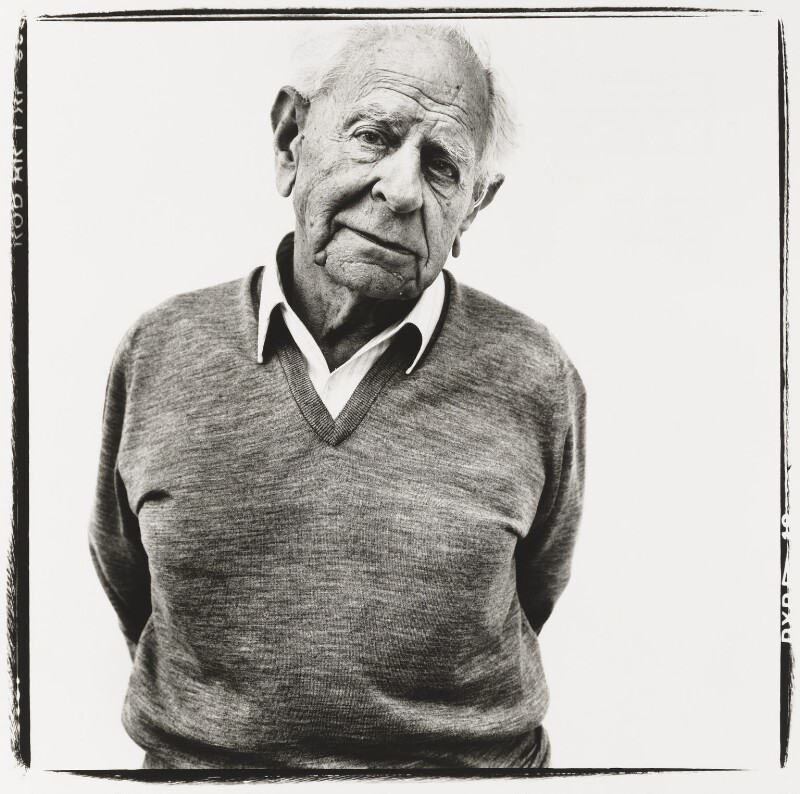
\includegraphics[width=0.5\textwidth]{images/karl-popper.png}

  \legend{Source: \href{https://www.npg.org.uk/collections/search/portrait/mw08238/Sir-Karl-Raimund-Popper?}{Steve Pyke}.}
\end{figure}

\hypertarget{secondary-section}{%
\section{Secondary section}\label{secondary-section}}

\begin{Shaded}
\begin{Highlighting}[numbers=left,,]
\CommentTok{\# library(datasets)}
\CommentTok{\# library(dplyr)}

\NormalTok{datasets}\SpecialCharTok{::}\NormalTok{iris }\SpecialCharTok{|\textgreater{}}
\NormalTok{  dplyr}\SpecialCharTok{::}\FunctionTok{as\_tibble}\NormalTok{() }\SpecialCharTok{|\textgreater{}}
\NormalTok{  dplyr}\SpecialCharTok{::}\FunctionTok{slice\_sample}\NormalTok{(}\AttributeTok{n =} \DecValTok{5}\NormalTok{) }\SpecialCharTok{|\textgreater{}}
\NormalTok{  gt}\SpecialCharTok{::}\FunctionTok{gt}\NormalTok{()}
\end{Highlighting}
\end{Shaded}

\hypertarget{tbl-iris}{}
\begin{longtable}{rrrrc}
\caption{\label{tbl-iris}A sample of the famous (Fisher's or Anderson's) iris data set }\tabularnewline

\toprule
Sepal.Length & Sepal.Width & Petal.Length & Petal.Width & Species \\ 
\midrule\addlinespace[2.5pt]
6.5 & 3.0 & 5.5 & 1.8 & virginica \\ 
6.5 & 3.0 & 5.8 & 2.2 & virginica \\ 
5.0 & 3.0 & 1.6 & 0.2 & setosa \\ 
5.0 & 3.5 & 1.6 & 0.6 & setosa \\ 
6.2 & 2.9 & 4.3 & 1.3 & versicolor \\ 
\bottomrule
\end{longtable}

\hypertarget{tertiary-section}{%
\subsection{Tertiary section}\label{tertiary-section}}

\begin{Shaded}
\begin{Highlighting}[numbers=left,,]
\CommentTok{\# library(datasets)}
\CommentTok{\# library(ggplot2)}

\NormalTok{ggplot2}\SpecialCharTok{::}\FunctionTok{ggplot}\NormalTok{(faithful, ggplot2}\SpecialCharTok{::}\FunctionTok{aes}\NormalTok{(}\AttributeTok{x =}\NormalTok{ eruptions, }\AttributeTok{y =}\NormalTok{ waiting)) }\SpecialCharTok{+}
\NormalTok{  ggplot2}\SpecialCharTok{::}\FunctionTok{geom\_point}\NormalTok{() }\SpecialCharTok{+}
\NormalTok{  ggplot2}\SpecialCharTok{::}\FunctionTok{xlim}\NormalTok{(}\FloatTok{0.5}\NormalTok{, }\DecValTok{6}\NormalTok{) }\SpecialCharTok{+}
\NormalTok{  ggplot2}\SpecialCharTok{::}\FunctionTok{ylim}\NormalTok{(}\DecValTok{40}\NormalTok{, }\DecValTok{110}\NormalTok{) }\SpecialCharTok{+}
\NormalTok{  ggplot2}\SpecialCharTok{::}\FunctionTok{geom\_density\_2d\_filled}\NormalTok{(}\AttributeTok{alpha =} \FloatTok{0.5}\NormalTok{) }\SpecialCharTok{+}
\NormalTok{  ggplot2}\SpecialCharTok{::}\FunctionTok{geom\_density\_2d}\NormalTok{(}\AttributeTok{linewidth =} \FloatTok{0.25}\NormalTok{, }\AttributeTok{colour =} \StringTok{"black"}\NormalTok{) }\SpecialCharTok{+}
\NormalTok{  ggplot2}\SpecialCharTok{::}\FunctionTok{theme}\NormalTok{(}\AttributeTok{legend.position =} \StringTok{"none"}\NormalTok{)}
\end{Highlighting}
\end{Shaded}

\begin{figure}[H]

\caption{\label{fig-eruption}Relationship between \emph{waiting time to
next eruption} (minutes) and \emph{eruption time} (minutes) at Old
Faithful Geyser, Yellowstone National Park, Wyoming, USA.}

{\centering 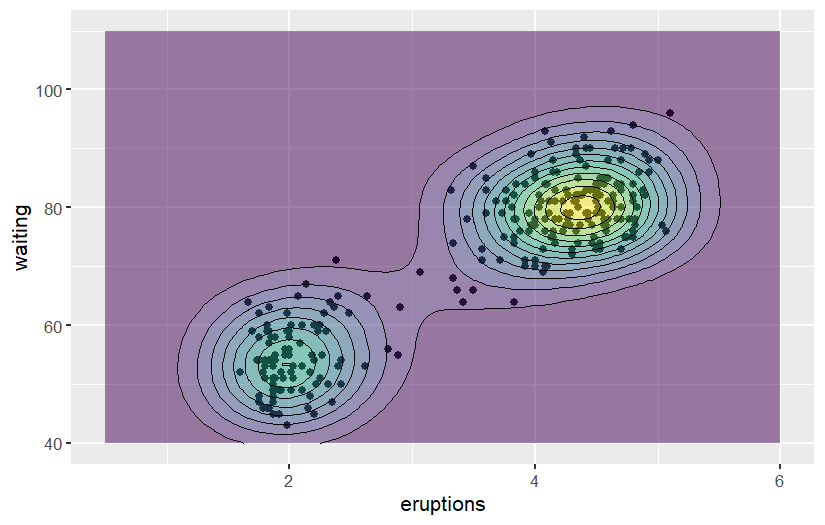
\includegraphics{index_files/figure-pdf/fig-eruption-1.png}

}

\end{figure}

\clearpage

\hypertarget{quaternary-section}{%
\subsubsection{Quaternary section}\label{quaternary-section}}

\begin{itemize}
\tightlist
\item
  Bullet point

  \begin{itemize}
  \tightlist
  \item
    Bullet point

    \begin{itemize}
    \tightlist
    \item
      Bullet point
    \end{itemize}
  \end{itemize}
\end{itemize}

\hypertarget{quinary-section}{%
\paragraph{Quinary section}\label{quinary-section}}

\begin{enumerate}
\def\labelenumi{\arabic{enumi}.}
\tightlist
\item
  List
\item
  List
\item
  List
\end{enumerate}

\begin{Shaded}
\begin{Highlighting}[numbers=left,,]
\CommentTok{\# library(ggplot2)}

\NormalTok{ggplot2}\SpecialCharTok{::}\FunctionTok{ggplot}\NormalTok{(ggplot2}\SpecialCharTok{::}\NormalTok{diamonds, ggplot2}\SpecialCharTok{::}\FunctionTok{aes}\NormalTok{(carat, price)) }\SpecialCharTok{+}
\NormalTok{  ggplot2}\SpecialCharTok{::}\FunctionTok{geom\_boxplot}\NormalTok{(ggplot2}\SpecialCharTok{::}\FunctionTok{aes}\NormalTok{(}\AttributeTok{group =}\NormalTok{ ggplot2}\SpecialCharTok{::}\FunctionTok{cut\_width}\NormalTok{(carat, }\FloatTok{0.25}\NormalTok{)))}
\end{Highlighting}
\end{Shaded}

\begin{figure}[H]

\caption{\label{fig-diamonds}Relations betwwen \emph{price} and
\emph{carat} (weight) of diamonds.}

{\centering 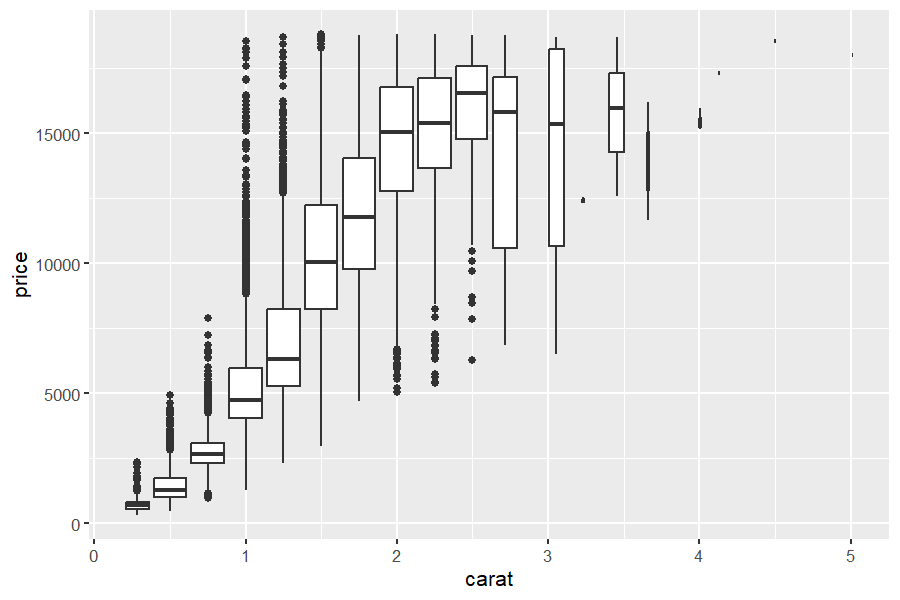
\includegraphics{index_files/figure-pdf/fig-diamonds-1.png}

}

\end{figure}

\bookmarksetup{startatroot}

\hypertarget{showcase-development}{%
\chapter{{[}Showcase{]} Development}\label{showcase-development}}

\begin{tcolorbox}[enhanced jigsaw, left=2mm, coltitle=black, breakable, bottomrule=.15mm, colbacktitle=quarto-callout-warning-color!10!white, opacitybacktitle=0.6, arc=.35mm, leftrule=.75mm, titlerule=0mm, rightrule=.15mm, colframe=quarto-callout-warning-color-frame, toprule=.15mm, title=\textcolor{quarto-callout-warning-color}{\faExclamationTriangle}\hspace{0.5em}{Warning}, opacityback=0, toptitle=1mm, colback=white, bottomtitle=1mm]

The text below is for demonstrative purposes only.

\vspace{0.25\baselineskip}

See \url{https://github.com/danielvartan/abnt} to learn more about this
template.

\end{tcolorbox}

Cillum qui eu non ipsum pariatur ad exercitation pariatur dolore veniam
amet cillum. Aliqua do nostrud aliquip in amet. Commodo sit tempor nulla
ipsum officia voluptate laborum elit minim proident Lorem. Id pariatur
reprehenderit non officia fugiat incididunt anim aliquip anim anim.
Ipsum irure magna quis est aute. Nostrud nulla mollit non labore. In
laboris mollit ea in. Excepteur eu do elit proident. Commodo tempor nisi
enim ex velit voluptate dolor mollit eiusmod in ullamco aliqua nostrud
id.

Eiusmod dolore sint proident consectetur reprehenderit exercitation
sunt. Nisi qui sit commodo anim consectetur in laborum dolore in labore
veniam labore commodo tempor. Sunt sit officia commodo quis magna.
Aliqua esse est adipisicing ea est ex esse esse officia sit culpa minim
amet dolore. Culpa dolore laborum sunt do commodo duis in velit. Mollit
duis voluptate aliquip magna labore aute sit dolore amet culpa labore.
Id tempor consectetur est anim ullamco ex nostrud voluptate excepteur.
Aliqua laboris aute laborum amet eu. Minim quis veniam et dolor quis
fugiat. Adipisicing amet est do aliqua nostrud amet excepteur ut.

\hypertarget{secondary-section-1}{%
\section{Secondary section}\label{secondary-section-1}}

Minim consectetur eu aliqua in elit incididunt labore amet consequat
cillum minim. Id sit duis duis ex velit proident mollit minim consequat
nulla. Aliqua elit do excepteur nulla nostrud exercitation nisi tempor
incididunt. Veniam dolore in non nisi veniam aliquip. Minim labore
excepteur ea est dolore laboris cillum. Laboris sit pariatur pariatur
veniam mollit nisi cupidatat qui qui quis laborum veniam dolor. Proident
aliquip do adipisicing dolor elit aute elit. Officia anim quis id
voluptate eu. Quis labore consectetur est magna. Laborum nulla ea non
Lorem officia aute.

\bookmarksetup{startatroot}

\hypertarget{showcase-conclusion}{%
\chapter{{[}Showcase{]} Conclusion}\label{showcase-conclusion}}

\begin{tcolorbox}[enhanced jigsaw, left=2mm, coltitle=black, breakable, bottomrule=.15mm, colbacktitle=quarto-callout-important-color!10!white, opacitybacktitle=0.6, arc=.35mm, leftrule=.75mm, titlerule=0mm, rightrule=.15mm, colframe=quarto-callout-important-color-frame, toprule=.15mm, title=\textcolor{quarto-callout-important-color}{\faExclamation}\hspace{0.5em}{Important}, opacityback=0, toptitle=1mm, colback=white, bottomtitle=1mm]

The text below is for demonstrative purposes only.

\vspace{0.25\baselineskip}

See \url{https://github.com/danielvartan/abnt} to learn more about this
template.

\end{tcolorbox}

Cillum qui eu non ipsum pariatur ad exercitation pariatur dolore veniam
amet cillum. Aliqua do nostrud aliquip in amet. Commodo sit tempor nulla
ipsum officia voluptate laborum elit minim proident Lorem. Id pariatur
reprehenderit non officia fugiat incididunt anim aliquip anim anim.
Ipsum irure magna quis est aute. Nostrud nulla mollit non labore. In
laboris mollit ea in. Excepteur eu do elit proident. Commodo tempor nisi
enim ex velit voluptate dolor mollit eiusmod in ullamco aliqua nostrud
id.

Eiusmod dolore sint proident consectetur reprehenderit exercitation
sunt. Nisi qui sit commodo anim consectetur in laborum dolore in labore
veniam labore commodo tempor. Sunt sit officia commodo quis magna.
Aliqua esse est adipisicing ea est ex esse esse officia sit culpa minim
amet dolore. Culpa dolore laborum sunt do commodo duis in velit. Mollit
duis voluptate aliquip magna labore aute sit dolore amet culpa labore.
Id tempor consectetur est anim ullamco ex nostrud voluptate excepteur.
Aliqua laboris aute laborum amet eu. Minim quis veniam et dolor quis
fugiat. Adipisicing amet est do aliqua nostrud amet excepteur ut.

\hypertarget{secondary-section-2}{%
\section{Secondary section}\label{secondary-section-2}}

Minim consectetur eu aliqua in elit incididunt labore amet consequat
cillum minim. Id sit duis duis ex velit proident mollit minim consequat
nulla. Aliqua elit do excepteur nulla nostrud exercitation nisi tempor
incididunt. Veniam dolore in non nisi veniam aliquip. Minim labore
excepteur ea est dolore laboris cillum. Laboris sit pariatur pariatur
veniam mollit nisi cupidatat qui qui quis laborum veniam dolor. Proident
aliquip do adipisicing dolor elit aute elit. Officia anim quis id
voluptate eu. Quis labore consectetur est magna. Laborum nulla ea non
Lorem officia aute.

\postextual

\begingroup
\renewcommand{\baselinestretch}{1}
\setcounter{footnote}{0}
\renewcommand{\thefootnote}{\fnsymbol{footnote}}
\printbibliography[heading=bibheading]
\endgroup

\addtocontents{toc}{\protect\vspace{1em}}
\cftinserthook{toc}{bibhook}
\addcontentsline{toc}{chapter}{
  \protect\numberline{}
  \newbibname
  \hspace{-0.25em}
}

\begin{apendicesenv}

\cleardoublepage
\phantomsection
\addcontentsline{toc}{part}{Appendices}
\appendix

\hypertarget{showcase}{%
\chapter{{[}Showcase{]}}\label{showcase}}

\begin{tcolorbox}[enhanced jigsaw, left=2mm, coltitle=black, breakable, bottomrule=.15mm, colbacktitle=quarto-callout-tip-color!10!white, opacitybacktitle=0.6, arc=.35mm, leftrule=.75mm, titlerule=0mm, rightrule=.15mm, colframe=quarto-callout-tip-color-frame, toprule=.15mm, title=\textcolor{quarto-callout-tip-color}{\faLightbulb}\hspace{0.5em}{Tip}, opacityback=0, toptitle=1mm, colback=white, bottomtitle=1mm]

The text below is for demonstrative purposes only.

\vspace{0.25\baselineskip}

See \url{https://quarto.org/docs/authoring/markdown-basics.html} to
learn about the basics of Markdown's syntax.

\end{tcolorbox}

Cillum qui eu non ipsum pariatur ad exercitation pariatur dolore veniam
amet cillum. Aliqua do nostrud aliquip in amet. Commodo sit tempor nulla
ipsum officia voluptate laborum elit minim proident Lorem. Id pariatur
reprehenderit non officia fugiat incididunt anim aliquip anim anim.
Ipsum irure magna quis est aute. Nostrud nulla mollit non labore. In
laboris mollit ea in. Excepteur eu do elit proident. Commodo tempor nisi
enim ex velit voluptate dolor mollit eiusmod in ullamco aliqua nostrud
id.

Eiusmod dolore sint proident consectetur reprehenderit exercitation
sunt. Nisi qui sit commodo anim consectetur in laborum dolore in labore
veniam labore commodo tempor. Sunt sit officia commodo quis magna.
Aliqua esse est adipisicing ea est ex esse esse officia sit culpa minim
amet dolore. Culpa dolore laborum sunt do commodo duis in velit. Mollit
duis voluptate aliquip magna labore aute sit dolore amet culpa labore.
Id tempor consectetur est anim ullamco ex nostrud voluptate excepteur.
Aliqua laboris aute laborum amet eu. Minim quis veniam et dolor quis
fugiat. Adipisicing amet est do aliqua nostrud amet excepteur ut.

\hypertarget{secondary-section-3}{%
\section{Secondary section}\label{secondary-section-3}}

Minim consectetur eu aliqua in elit incididunt labore amet consequat
cillum minim. Id sit duis duis ex velit proident mollit minim consequat
nulla. Aliqua elit do excepteur nulla nostrud exercitation nisi tempor
incididunt. Veniam dolore in non nisi veniam aliquip. Minim labore
excepteur ea est dolore laboris cillum. Laboris sit pariatur pariatur
veniam mollit nisi cupidatat qui qui quis laborum veniam dolor. Proident
aliquip do adipisicing dolor elit aute elit. Officia anim quis id
voluptate eu. Quis labore consectetur est magna. Laborum nulla ea non
Lorem officia aute.

\hypertarget{settings}{%
\chapter{Settings}\label{settings}}

\begin{tcolorbox}[enhanced jigsaw, left=2mm, coltitle=black, breakable, bottomrule=.15mm, colbacktitle=quarto-callout-important-color!10!white, opacitybacktitle=0.6, arc=.35mm, leftrule=.75mm, titlerule=0mm, rightrule=.15mm, colframe=quarto-callout-important-color-frame, toprule=.15mm, title=\textcolor{quarto-callout-important-color}{\faExclamation}\hspace{0.5em}{Important}, opacityback=0, toptitle=1mm, colback=white, bottomtitle=1mm]

You are reading the work-in-progress of this manual.

\vspace{0.25\baselineskip}

This chapter is undergoing heavy restructuring and may be confusing or
incomplete.

\end{tcolorbox}

\hypertarget{typography}{%
\section{Typography}\label{typography}}

\hypertarget{typeface}{%
\subsection{Typeface}\label{typeface}}

To change typefaces, simply use the
\href{https://quarto.org/docs/reference/formats/pdf.html}{Quarto
options}, such as \texttt{mainfont}, \texttt{monofont} and
\texttt{sansfont} in your \texttt{quarto-{[}format{]}.yml} file.

\begin{Shaded}
\begin{Highlighting}[numbers=left,,]
\FunctionTok{format}\KeywordTok{:}
\AttributeTok{  }\FunctionTok{abnt{-}pdf}\KeywordTok{:}
\AttributeTok{    }\FunctionTok{mainfont}\KeywordTok{:}\AttributeTok{ Arial}
\end{Highlighting}
\end{Shaded}

The ABNT NBR 14724:2011 norm does not specify the use of any specific
font. You have the freedom to choose any font you prefer, but it's
important to note that the selected font must be installed on your
computer.

\hypertarget{font-size}{%
\subsection{Font size}\label{font-size}}

To adjust the font size, utilize the \texttt{fontsize} option in in the
\texttt{quarto-{[}format{]}.yml} file.

\begin{Shaded}
\begin{Highlighting}[numbers=left,,]
\FunctionTok{format}\KeywordTok{:}
\AttributeTok{  }\FunctionTok{abnt{-}pdf}\KeywordTok{:}
\AttributeTok{    }\FunctionTok{fontsize}\KeywordTok{:}\AttributeTok{ 12pt}
\end{Highlighting}
\end{Shaded}

It's important to note that the third paragraph of Section 5.1 of ABNT
NBR 14724:2011 norm establishes that the font size should be 12pt for
the entire document, including the cover, except for quotations longer
than three lines, footnotes, pagination, cataloging data, captions, and
sources of illustrations and tables, which should be in a smaller and
uniform size.

The smaller font is set to \texttt{\textbackslash{}footnotesize}, which
corresponds to a 10pt font size with the default settings. You can
modify this setting by inserting the following LaTeX command into
\texttt{tex/include-in-header.tex}:

\begin{Shaded}
\begin{Highlighting}[numbers=left,,]
\FunctionTok{\textbackslash{}renewcommand}\NormalTok{\{}\ExtensionTok{\textbackslash{}ABNTEXfontereduzida}\NormalTok{\}\{[NEW SIZE (e.g., }\FunctionTok{\textbackslash{}small}\NormalTok{)]\}}
\end{Highlighting}
\end{Shaded}

\hypertarget{language-and-hyphenation}{%
\section{Language and hyphenation}\label{language-and-hyphenation}}

\hypertarget{document-sections}{%
\section{Document sections}\label{document-sections}}

\hypertarget{editing-pre-textual-sections}{%
\subsection{Editing pre-textual
sections}\label{editing-pre-textual-sections}}

\texttt{abnt} uses a system of tags to transfer and render the content
of Quarto files (\texttt{.qmd}) to LaTeX. These tags look like this:

\begin{Shaded}
\begin{Highlighting}[numbers=left,,]
\CommentTok{\%:::\% class attribute begin/end \%:::\%}
\end{Highlighting}
\end{Shaded}

\begin{Shaded}
\begin{Highlighting}[numbers=left,,]
\CommentTok{\textless{}!{-}{-} \%:::\% class attribute begin/end \%:::\% {-}{-}\textgreater{}}
\end{Highlighting}
\end{Shaded}

Unless you want to customize the template, you don't need to modify the
\texttt{.tex} files. You can write directly in the \texttt{.qmd} files.
Just ensure that you preserve all the tags.

\hypertarget{how-to-include-latex-commands-in-quarto-files-.qmd}{%
\subsection{\texorpdfstring{How to include LaTeX commands in Quarto
files
(\texttt{.qmd})}{How to include LaTeX commands in Quarto files (.qmd)}}\label{how-to-include-latex-commands-in-quarto-files-.qmd}}

To add LaTeX commands in your writing, without worrying that it will
contaminate the \texttt{html} format, use a \texttt{\{=latex\}} chunk.

\begin{Shaded}
\begin{Highlighting}[numbers=left,,]
\FunctionTok{\textbackslash{}\textasciigrave{}}\NormalTok{\textasciigrave{}\textasciigrave{}\{=latex\}}
\CommentTok{\% Some LaTeX code.}
\FunctionTok{\textbackslash{}\textasciigrave{}}\NormalTok{\textasciigrave{}\textasciigrave{}}
\end{Highlighting}
\end{Shaded}

\hypertarget{how-to-add-or-remove-sections}{%
\subsection{How to add or remove
sections}\label{how-to-add-or-remove-sections}}

For pre-textual sections (e.g., list of symbols, abstract), remove them
from \texttt{tex/include-before-body.tex} and from
\texttt{R/quarto-pre-render.R}.

For textual sections (e.g., chapters), remove them from the
\texttt{.quarto-{[}format{]}.yml} file.

For post-textual sections (e.g., appendices, annexes), if it's a
appendix, remove it from \texttt{.quarto-{[}format{]}.yml}; else, remove
them from \texttt{tex/include-after-body.tex}.

It's important to note that, at this moment, the last chapter must have
a LaTeX code chunk at the end of it. The same is true for the last
appendix chapter. They should look like this:

\begin{tcolorbox}[enhanced jigsaw, left=2mm, coltitle=black, breakable, bottomrule=.15mm, colbacktitle=quarto-callout-warning-color!10!white, opacitybacktitle=0.6, arc=.35mm, leftrule=.75mm, titlerule=0mm, rightrule=.15mm, colframe=quarto-callout-warning-color-frame, toprule=.15mm, title=\textcolor{quarto-callout-warning-color}{\faExclamationTriangle}\hspace{0.5em}{Warning}, opacityback=0, toptitle=1mm, colback=white, bottomtitle=1mm]

Remove the \texttt{\textbackslash{}} from the beginning and end of the
code below when applying it.

\end{tcolorbox}

\begin{Shaded}
\begin{Highlighting}[numbers=left,,]
\FunctionTok{\textbackslash{}\textasciigrave{}}\NormalTok{\textasciigrave{}\textasciigrave{}\{=latex\}}
\FunctionTok{\textbackslash{}postextual}

\FunctionTok{\textbackslash{}begingroup}
\FunctionTok{\textbackslash{}renewcommand}\NormalTok{\{}\ExtensionTok{\textbackslash{}baselinestretch}\NormalTok{\}\{1\}}
\FunctionTok{\textbackslash{}setcounter}\NormalTok{\{footnote\}\{0\}}
\FunctionTok{\textbackslash{}renewcommand}\NormalTok{\{}\ExtensionTok{\textbackslash{}thefootnote}\NormalTok{\}\{}\FunctionTok{\textbackslash{}fnsymbol}\NormalTok{\{footnote\}\}}
\FunctionTok{\textbackslash{}printbibliography}\NormalTok{[heading=bibheading]}
\FunctionTok{\textbackslash{}endgroup}

\FunctionTok{\textbackslash{}addtocontents}\NormalTok{\{toc\}\{}\FunctionTok{\textbackslash{}protect\textbackslash{}vspace}\NormalTok{\{1em\}\}}
\FunctionTok{\textbackslash{}cftinserthook}\NormalTok{\{toc\}\{bibhook\}}
\FunctionTok{\textbackslash{}addcontentsline}\NormalTok{\{toc\}\{chapter\}\{}
  \FunctionTok{\textbackslash{}protect\textbackslash{}numberline}\NormalTok{\{\}}
  \FunctionTok{\textbackslash{}newbibname}
  \FunctionTok{\textbackslash{}hspace}\NormalTok{\{{-}0.25em\}}
\NormalTok{\}}

\KeywordTok{\textbackslash{}begin}\NormalTok{\{}\ExtensionTok{apendicesenv}\NormalTok{\}}
\FunctionTok{\textbackslash{}\textasciigrave{}}\NormalTok{\textasciigrave{}\textasciigrave{}}
\end{Highlighting}
\end{Shaded}

\begin{Shaded}
\begin{Highlighting}[numbers=left,,]
\FunctionTok{\textbackslash{}\textasciigrave{}}\NormalTok{\textasciigrave{}\textasciigrave{} \{=latex\}}
\KeywordTok{\textbackslash{}end}\NormalTok{\{}\ExtensionTok{apendicesenv}\NormalTok{\}}
\FunctionTok{\textbackslash{}\textasciigrave{}}\NormalTok{\textasciigrave{}\textasciigrave{}}
\end{Highlighting}
\end{Shaded}

\hypertarget{citation-management}{%
\section{Citation management}\label{citation-management}}

\hypertarget{citation-method}{%
\subsection{Citation method}\label{citation-method}}

This Quarto format was specifically designed to be compatible with
\href{https://www.ctan.org/pkg/biblatex}{BibLaTeX}, which is a
comprehensive reimplementation of
\href{https://www.bibtex.org/}{BiBTeX}. At first glance, these two
systems may appear very similar.

To get started, simply insert your references into the
\texttt{references.bib}file. However, this task can be somewhat tedious
and demanding. To simplify the process, we recommend exploring the
integration of \href{https://www.zotero.org/}{Zotero} along with
\href{https://github.com/retorquere/zotero-better-bibtex}{Better
BiBTeX}, as demonstrated in a section below.

For detailed guidance on handling citations in Quarto, please refer to
Quarto's
\href{https://quarto.org/docs/authoring/footnotes-and-citations.html}{Citation
\& Footnotes} documentation.

\hypertarget{citation-style}{%
\subsection{Citation style}\label{citation-style}}

There are two built-in citation styles:

\begin{itemize}
\tightlist
\item
  \href{https://www.abnt.org.br/}{ABNT} (Brazilian Association of
  Technical Standards);
\item
  \href{https://apastyle.apa.org/}{APA} (American Psychological
  Association).
\end{itemize}

To use one of them, simply change the \texttt{biblio-style} option in
your \texttt{yml} file with the style of you preference.

\begin{Shaded}
\begin{Highlighting}[numbers=left,,]
\FunctionTok{format}\KeywordTok{:}
\AttributeTok{  }\FunctionTok{abnt{-}pdf}\KeywordTok{:}
\AttributeTok{    }\FunctionTok{biblio{-}style}\KeywordTok{:}\AttributeTok{ abnt}\CommentTok{ \# options: [abnt, abnt{-}ibid, abnt{-}numeric, apa]}
\end{Highlighting}
\end{Shaded}

There are other options related to the citation style; some are shown
below. Please refer to
\href{https://www.ctan.org/pkg/biblatex}{\texttt{biblatex}},
\href{https://www.ctan.org/pkg/biblatex-abnt}{\texttt{biblatex-abnt}}
and \href{https://www.ctan.org/pkg/biblatex-apa}{\texttt{biblatex-apa}}
manuals to learn more about them.

\begin{Shaded}
\begin{Highlighting}[numbers=left,,]
\FunctionTok{format}\KeywordTok{:}
\AttributeTok{  }\FunctionTok{abnt{-}pdf}\KeywordTok{:}
\FunctionTok{    biblio{-}footnote}\KeywordTok{: }\CharTok{\textgreater{}}
\NormalTok{      According to the Brazilian Association of Technical Standards}
\NormalTok{      (ABNT NBR 6023).}
\AttributeTok{    }\FunctionTok{biblatexoptions}\KeywordTok{:}
\AttributeTok{      }\KeywordTok{{-}}\AttributeTok{ backend=biber,}
\AttributeTok{      }\KeywordTok{{-}}\AttributeTok{ language=english,}\CommentTok{ \# [options: english, brazil, spanish, french]}
\AttributeTok{      }\KeywordTok{{-}}\AttributeTok{ url=true,}
\AttributeTok{      }\KeywordTok{{-}}\AttributeTok{ useprefix=false,}
\AttributeTok{      }\KeywordTok{{-}}\AttributeTok{ giveninits=true,}
\AttributeTok{      }\KeywordTok{{-}}\AttributeTok{ extrayear=true}
\AttributeTok{    }\FunctionTok{bibhang}\KeywordTok{:}\AttributeTok{ 0cm}\CommentTok{ \# Use 0.5cm if \textasciigrave{}biblio{-}style: apa\textasciigrave{}.}
\AttributeTok{    }\FunctionTok{bibparsep}\KeywordTok{:}\AttributeTok{ 0ex}
\end{Highlighting}
\end{Shaded}

\hypertarget{zotero-integration}{%
\subsection{Zotero integration}\label{zotero-integration}}

This template can work with \href{https://www.zotero.org/}{Zotero} and
the \href{https://github.com/retorquere/zotero-better-bibtex}{Better
BiBTeX} plugin. The advantage of using this integration is that you
don't need to manually input your references into
\texttt{references.bib}; they are automatically imported when you render
the format.

For this to work, you must activate the \texttt{zotero} option in your
\texttt{yml} file and have Zotero, with Better BibTeX installed, open
while rendering your thesis. A pre-render script (see
\texttt{R/quarto-pre-render.R}), created using the
\href{https://github.com/paleolimbot/rbbt}{\texttt{rbbt}} R package,
will scan all \texttt{.qmd} and \texttt{.tex} files searching for BibTeX
citations (e.g., \texttt{@watson1953}). If they match with your Zotero
database, the citations will then be written into the
\texttt{references.bib} file.

\begin{Shaded}
\begin{Highlighting}[numbers=left,,]
\FunctionTok{format}\KeywordTok{:}
\AttributeTok{  }\FunctionTok{abnt{-}pdf}\KeywordTok{:}
\AttributeTok{    }\FunctionTok{zotero}\KeywordTok{:}\AttributeTok{ }\CharTok{true}
\end{Highlighting}
\end{Shaded}

\hypertarget{title-case-change}{%
\subsubsection{Title case change}\label{title-case-change}}

By using \href{https://www.zotero.org/}{Zotero}, you may experience a
title casing change when exporting your references. This is the default
behavior of \href{https://retorque.re/zotero-better-bibtex/}{Better
BibTex} while exporting to BibLaTeX.

You can disable this by going to Zotero's configuration editor (go to
Edit \textgreater{} Preferences \textgreater{} Advanced \textgreater{}
Config Editor) and changing the variable\textbackslash{}
\texttt{extensions.zotero.translators.better-bibtex.exportTitleCase} to
\texttt{false}. Beware that this can produce some issues. You can find
more information about this behavior
\href{https://retorque.re/zotero-better-bibtex/support/faq/\#bbt-is-changing-the-capitalization-of-my-titles----why}{here}.

\hypertarget{abnt-figures-and-tables}{%
\section{ABNT figures and tables}\label{abnt-figures-and-tables}}

(work in progress - consider adding a
\href{https://yihui.org/knitr/hooks/}{knitr hook})

\hypertarget{figures}{%
\subsection{Figures}\label{figures}}

See \href{https://quarto.org/docs/reference/cells/}{Code Cells}.

\begin{enumerate}
\def\labelenumi{(\arabic{enumi})}
\tightlist
\item
  Create a new figure environment.
\end{enumerate}

Name it \texttt{abntfigure} and include an
\texttt{\textbackslash{}quartolegend} in the end.

Use \texttt{\textbackslash{}notblank} from \texttt{etoolbox} package to
add a conditional layer.

\begin{enumerate}
\def\labelenumi{(\arabic{enumi})}
\setcounter{enumi}{1}
\tightlist
\item
  Add the new environment to \texttt{fig-env} in
  \texttt{\_extension.yml}.
\end{enumerate}

\hypertarget{tables}{%
\subsection{Tables}\label{tables}}

\begin{enumerate}
\def\labelenumi{\arabic{enumi}.}
\tightlist
\item
  Add a hook at the end of the \texttt{longtable} environment.
\end{enumerate}

Include the \texttt{\textbackslash{}quartolegend} and utilize
\texttt{\textbackslash{}notblank} from \texttt{etoolbox} package to add
a conditional layer.

\begin{Shaded}
\begin{Highlighting}[numbers=left,,]
\FunctionTok{\textbackslash{}AddToHook}\NormalTok{\{env/longtable/before\}\{\}}
\FunctionTok{\textbackslash{}AddToHook}\NormalTok{\{env/longtable/after\}\{\}}
\FunctionTok{\textbackslash{}AddToHook}\NormalTok{\{env/longtable/begin\}\{}
  \FunctionTok{\textbackslash{}ABNTEXfontereduzida}
  \FunctionTok{\textbackslash{}renewcommand}\NormalTok{\{}\ExtensionTok{\textbackslash{}arraystretch}\NormalTok{\}\{1\}}
\NormalTok{\}}
\FunctionTok{\textbackslash{}AddToHook}\NormalTok{\{env/longtable/end\}\{\}}
\end{Highlighting}
\end{Shaded}

\hypertarget{freezing-and-cache}{%
\section{Freezing and cache}\label{freezing-and-cache}}

See
\href{https://quarto.org/docs/projects/code-execution.html\#freeze}{Freeze}.

\hypertarget{how-to-customize-this-quarto-format}{%
\section{How to customize this Quarto
format}\label{how-to-customize-this-quarto-format}}

\hypertarget{quarto-system}{%
\subsection{Quarto system}\label{quarto-system}}

See \href{https://quarto.org/docs/guide/}{Quarto's guide}.

\hypertarget{template-and-template-partials}{%
\subsection{Template and template
partials}\label{template-and-template-partials}}

See
\href{https://quarto.org/docs/journals/templates.html\#template-partials}{Tempalte
partials}.

\hypertarget{spacing-rules}{%
\subsection{Spacing rules}\label{spacing-rules}}

\begin{itemize}
\tightlist
\item
  Set fixed dimensions (e.g., page dimensions) in \texttt{cm} or
  \texttt{pt}. \texttt{cm} is the prefer unit for margins.
\item
  Set line spacing as a proportion of
  \texttt{\textbackslash{}baselineskip} (e.g.,
  \texttt{1.5\textbackslash{}baselineskip}).
\item
  Use the settings \texttt{\textbackslash{}tinyskipamount},
  \texttt{\textbackslash{}smallskipamount},
  \texttt{\textbackslash{}midskipamount},
  \texttt{\textbackslash{}bigskipamount},
  \texttt{\textbackslash{}hugeskipamount} and their counterparts
  \texttt{\textbackslash{}tinyskip}, \texttt{\textbackslash{}smallskip},
  \texttt{\textbackslash{}midskip}, \texttt{\textbackslash{}bigskip},
  \texttt{\textbackslash{}hugeskip}. You can find them in the
  \texttt{lengths.tex} template partial.
\item
  For other kinds of relative vertical spacing, use the \texttt{ex}
  unit.
\item
  For relative horizontal spacing, use the \texttt{em} unit.
\end{itemize}

See \textcite[section 7.5]{oetiker2023} to learn more about LaTeX
spacing features. The articles on
\href{https://www.overleaf.com}{Overleaf} are also a great source of
information. Check
\href{https://www.overleaf.com/learn/latex/Lengths_in_LaTeX}{Lengths in
LaTeX} and
\href{https://www.overleaf.com/learn/latex/Articles/How_to_change_paragraph_spacing_in_LaTeX}{How
to change paragraph spacing in LaTeX} to get a sense of the subject.

\hypertarget{unit-equivalences}{%
\subsubsection{Unit equivalences}\label{unit-equivalences}}

\begin{itemize}
\tightlist
\item
  1\texttt{em} \(==\) 12\texttt{pt} or \(\approx\)
  0.423333\$\texttt{cm}.
\item
  1\texttt{ex} \(==\) \(\approx\) 6.22266\texttt{pt} or \(\approx\)
  0.219521\texttt{cm}.
\end{itemize}

\hypertarget{baselineskip}{%
\paragraph{\texorpdfstring{\texttt{\textbackslash{}baselineskip}}{\textbackslash baselineskip}}\label{baselineskip}}

These are the equivalences for a Arial typeface with size 12\texttt{pt}:

Use \texttt{\textbackslash{}the\textbackslash{}baselineskip} and
\texttt{\textbackslash{}gevalue\{\}} to figure out the exact value. Note
that \texttt{\textbackslash{}gevalue\{\}} will return the value in
\texttt{pt}.

Example of using \texttt{\textbackslash{}getvalue\{\}}:

\begin{Shaded}
\begin{Highlighting}[numbers=left,,]
\FunctionTok{\textbackslash{}begingroup}
\FunctionTok{\textbackslash{}setlength}\NormalTok{\{}\FunctionTok{\textbackslash{}parskip}\NormalTok{\}\{1em\}}
\FunctionTok{\textbackslash{}getlength}\NormalTok{\{}\FunctionTok{\textbackslash{}parskip}\NormalTok{\}}
\FunctionTok{\textbackslash{}endgroup}
\end{Highlighting}
\end{Shaded}

\hypertarget{linestretch1}{%
\subparagraph{\texorpdfstring{\texttt{\textbackslash{}linestretch=1}}{\textbackslash linestretch=1}}\label{linestretch1}}

\begin{itemize}
\tightlist
\item
  \texttt{1\textbackslash{}baselineskip} \(==\) 14.5\texttt{pt}. That's
  about 1.2x (or (\$\approx\$1.208333x) the font size (standard
  procedure).
\end{itemize}

\hypertarget{linestretch1.5}{%
\subparagraph{\texorpdfstring{\texttt{\textbackslash{}linestretch=1.5}}{\textbackslash linestretch=1.5}}\label{linestretch1.5}}

\begin{itemize}
\tightlist
\item
  \texttt{0.25\textbackslash{}baselineskip} \(==\) 5.4375\texttt{pt} or
  \(\approx\) 0.191822917\texttt{cm};
\item
  \texttt{0.5\textbackslash{}baselineskip} \(==\) 10.875\texttt{pt} or
  \(\approx\) 0.383645833\texttt{cm};
\item
  \texttt{0.75\textbackslash{}baselineskip} \(==\) 16.3125\texttt{pt} or
  \(\approx\) 0.57546875\texttt{cm};
\item
  \texttt{1\textbackslash{}baselineskip} \(==\) 21.75\texttt{pt} or
  \(\approx\) 0.76729167\texttt{cm};
\item
  \texttt{1.5\textbackslash{}baselineskip} \(==\) 32.625\texttt{pt} or
  \(\approx\) 1.1509375\texttt{cm};
\item
  \texttt{2\textbackslash{}baselineskip} \(==\) 43.5\texttt{pt} or
  \(\approx\) 1.534583\texttt{cm};
\item
  \texttt{2.5\textbackslash{}baselineskip} \(==\) 54.375\texttt{pt} or
  \(\approx\) 1.91822917\texttt{cm};
\item
  \texttt{3\textbackslash{}baselineskip} \(==\) 65.25\texttt{pt} or
  \(\approx\) 2.301875\texttt{cm}.
\end{itemize}

\hypertarget{how-to-add-new-citation-styles}{%
\subsection{How to add new citation
styles}\label{how-to-add-new-citation-styles}}

\hypertarget{must-see-references}{%
\subsection{Must see references}\label{must-see-references}}

To learn the basics about LaTeX, see \textcite{oetiker2023}. To delve
deeper into the LaTeX system, see \textcite{lamport1994} and
\textcite{knuth1986}.

\hypertarget{manuals}{%
\subsubsection{Manuals}\label{manuals}}

\begin{itemize}
\tightlist
\item
  \href{https://quarto.org/docs/guide/}{Quarto};
\item
  \href{https://www.ctan.org/pkg/abntex2}{\texttt{abntex2}};
\item
  \href{https://www.ctan.org/pkg/memoir}{\texttt{memoir}};
\item
  \href{https://www.ctan.org/pkg/biblatex}{\texttt{biblatex}};
\end{itemize}

\begin{itemize}
\tightlist
\item
  \href{https://www.ctan.org/pkg/biblatex-abnt}{\texttt{biblatex-abnt}};
\item
  \href{https://www.ctan.org/pkg/biblatex-apa}{\texttt{biblatex-apa}};
\item
  \href{https://ctan.org/pkg/babel}{\texttt{babel}};
\item
  \href{https://ctan.org/pkg/fontspec}{\texttt{fontspec}}.
\end{itemize}

\hypertarget{r-packages}{%
\subsubsection{R packages}\label{r-packages}}

\begin{itemize}
\tightlist
\item
  \href{https://gt.rstudio.com}{\texttt{gt}};
\end{itemize}

\begin{itemize}
\tightlist
\item
  \href{https://github.com/danielvartan/rutils/blob/main/R/quarto.R}{\texttt{rutils}}.
\end{itemize}

\end{apendicesenv}

% -----
% Attachments (optional)
% -----

\begin{anexosenv}
\chapter{(Showcase)}

Lorem ipsum dolor sit amet, consectetur adipiscing elit. Pellentesque accumsan rutrum lacus, vitae iaculis nisi bibendum in. Nulla et pellentesque nisl. Proin mollis dui sit amet egestas fermentum. Maecenas eu odio odio. Aenean porta ipsum in mauris pharetra dapibus. Nunc dapibus libero nec dui lacinia, id ultricies lectus maximus. Mauris quis mauris in velit pulvinar rutrum. Cras congue ante in orci luctus placerat. Nullam sit amet nisi augue. Maecenas non ligula eros. Etiam nec dolor a mi bibendum auctor.

\clearpage

\includepdf{images/anx_1.pdf}
\end{anexosenv}

% % -----
% % Index (optional)
% % -----
%
% % Use `index: true` below the `format: pdf:` to activated this section.
% % See <https://quarto.org/docs/books/book-structure.html#creating-an-index>
% %   to learn more.
%
% \phantompart
% \printindex

\end{document}
